% ============================================================
%  FitLabs - TFG DAM 2025-2026
%  Archivo principal - compilar con pdflatex o en Overleaf
% ============================================================
\documentclass[12pt,a4paper]{report}

% --- Codificación y fuentes ----------------------------------
\usepackage[T1]{fontenc}
\usepackage[utf8]{inputenc}
\usepackage{helvet}          % Helvetica ≈ Arial
\renewcommand{\familydefault}{\sfdefault}

% --- Idioma --------------------------------------------------
\usepackage[spanish]{babel}

% --- Márgenes 2.5 cm ----------------------------------------
\usepackage[top=2.5cm, bottom=2.5cm, left=2.5cm, right=2.5cm]{geometry}

% --- Interlineado 1.5 ----------------------------------------
\usepackage{setspace}
\onehalfspacing

% --- Encabezado y pie de página ------------------------------
\usepackage{fancyhdr}
\pagestyle{fancy}
\fancyhf{}
\fancyhead[L]{\footnotesize FitLabs -- TFG DAM 2025-2026}
\fancyhead[R]{\footnotesize J.L. Sánchez González \& C. Fraidias del Valle}
\fancyfoot[C]{\thepage}
\renewcommand{\headrulewidth}{0.4pt}

% --- Colores y gráficos --------------------------------------
\usepackage{xcolor}
\usepackage{graphicx}
\usepackage{float}
\graphicspath{{./imagenes/}}

% --- Tablas mejoradas ----------------------------------------
\usepackage{booktabs}
\usepackage{array}
\usepackage{longtable}
\usepackage{multirow}

% --- Código fuente -------------------------------------------
\usepackage{listings}
\lstset{
  basicstyle=\footnotesize\ttfamily,
  frame=single,
  breaklines=true,
  numbers=left,
  stepnumber=1,
  numberstyle=\tiny,
  keywordstyle=\bfseries\color{blue!70!black},
  commentstyle=\itshape\color{gray},
  stringstyle=\color{red!70!black},
}

% --- Hiperenlaces --------------------------------------------
\usepackage[hidelinks]{hyperref}
\usepackage{url}

% --- Listas --------------------------------------------------
\usepackage{enumitem}

% --- Citas ---------------------------------------------------
\usepackage{csquotes}
\usepackage[style=apa, backend=biber]{biblatex}
\addbibresource{bibliografia.bib}

% --- Diagrama de Gantt inline --------------------------------
\usepackage{pgfgantt}

% --- Colores personalizados FitLabs -------------------------
\definecolor{fitlabsPurple}{HTML}{3D2B6B}
\definecolor{fitlabsLight}{HTML}{9B7FD4}

% ============================================================
\begin{document}

% Numeración romana para portada e índice
\pagenumbering{roman}
\thispagestyle{empty}

% ---- PORTADA -----------------------------------------------
\begin{titlepage}
  \centering
  \vspace*{1cm}
  {\Huge \textbf{\textcolor{fitlabsPurple}{FitLabs}}}\\[0.3cm]
  {\large \textit{Aplicación Móvil para la Gestión Integral de Entrenadores Personales}}\\[2cm]

  
\includegraphics[width=5cm]{logo_fitlabs.png}\par
  \vspace{1.5cm}

  {\large \textbf{Autores}}\\[0.2cm]
  {\large José Luis Sánchez González \& Carlos Fraidias del Valle}\\[1cm]

  {\large \textbf{Tutor}}\\[0.2cm]
  {\large José Manuel Ruiz González}\\[1cm]

  {\large \textbf{Ciclo Formativo}}\\[0.2cm]
  {\large Desarrollo de Aplicaciones Multiplataforma (DAM)}\\[0.5cm]
  {\large Curso 2025 -- 2026}\\[2cm]

  \vfill
  {\small Trabajo de Final de Ciclo -- 4 de mayo de 2026}
\end{titlepage}

% ---- ÍNDICE ------------------------------------------------
\tableofcontents
\clearpage
\pagenumbering{arabic}
\setcounter{page}{1}

% ============================================================
% CAPÍTULOS
% ============================================================
% ============================================================
%  CAPÍTULO 3 – Análisis del Sector Productivo y Contexto Profesional
% ============================================================
\chapter{Análisis del Sector Productivo y Contexto Profesional}

\section{Descripción general del sector TIC}

El sector de las Tecnologías de la Información y la Comunicación (TIC) constituye actualmente uno de los motores económicos más dinámicos a escala mundial. Según datos recientes del INE, el número de empresas tecnológicas activas en España supera las 45\,000, con un crecimiento sostenido del empleo especializado superior al 6\,\% anual. El desarrollo de aplicaciones móviles ocupa un papel protagonista dentro de este ecosistema, impulsado por la masificación del uso de smartphones y la digitalización de sectores tan variados como la salud, el deporte o la educación.

En este contexto, las aplicaciones \textit{multiplataforma} han ganado una relevancia especial, ya que permiten llegar simultáneamente a dispositivos Android e iOS con una única base de código, reduciendo costes y acortando los tiempos de salida al mercado.

% TODO: Ampliar con estadísticas adicionales del sector fitness-tech (mercado global, facturación, tendencias de crecimiento). Fuentes recomendadas: Statista, Grand View Research.

\section{Tipos de empresas y áreas de actividad}

FitLabs encaja en la categoría de \textbf{aplicaciones de salud y bienestar personal} (Health \& Fitness Apps), un segmento que combina empresas de desarrollo de software con estudios de diseño UX/UI, empresas de servicios deportivos y startups tecnológicas especializadas. En un entorno comercial real, un producto como FitLabs podría ser desarrollado por:

\begin{itemize}
  \item Una startup de fitness-tech de tamaño reducido (3--10 personas).
  \item El departamento TI interno de una cadena de gimnasios.
  \item Una empresa de software a medida contratada por un colectivo de entrenadores personales.
\end{itemize}

Las áreas de actividad principales que intervienen en el ciclo de vida de la aplicación son: análisis de requisitos, diseño UI/UX, desarrollo frontend (Flutter), diseño de base de datos (Supabase/PostgreSQL), integración de APIs externas y garantía de calidad (QA).

\section{Necesidades actuales del mercado}

Los entrenadores personales operan habitualmente con herramientas genéricas (hojas de cálculo, WhatsApp, aplicaciones de notas) que resultan ineficientes para la gestión profesional de múltiples clientes. El mercado demanda soluciones que centralicen:

\begin{enumerate}
  \item La comunicación en tiempo real con los clientes.
  \item La creación y asignación de rutinas de entrenamiento personalizadas.
  \item El seguimiento del progreso físico de cada cliente.
  \item La organización del calendario de sesiones.
\end{enumerate}

FitLabs responde directamente a estas necesidades mediante una interfaz unificada y accesible desde cualquier dispositivo móvil.

\section{Oportunidades profesionales y de negocio}

La tendencia hacia un estilo de vida más activo y consciente de la salud, reforzada tras la pandemia de COVID-19, ha disparado la demanda de entrenadores personales y, por extensión, de herramientas digitales que les ayuden a gestionar sus servicios. Las tendencias más relevantes para el posicionamiento de FitLabs son:

\begin{itemize}
  \item \textbf{Entrenamiento online}: La modalidad de entrenamiento remoto ha consolidado la necesidad de plataformas digitales de gestión.
  \item \textbf{Wearables e IoT}: Integración futura con dispositivos de monitorización de la actividad física.
  \item \textbf{Personalización mediante IA}: Recomendación automática de rutinas basadas en el historial del cliente.
\end{itemize}

% TODO: Incluir datos de crecimiento del mercado fitness-tech en España y Europa para los años 2024-2026.

\section{Aspectos legales y de seguridad}

El proyecto maneja datos personales sensibles (datos de salud, actividad física, comunicaciones privadas), por lo que debe cumplir con la normativa vigente:

\begin{itemize}
  \item \textbf{RGPD} (Reglamento General de Protección de Datos, UE 2016/679): Los datos de los usuarios se almacenan en Supabase con cifrado en tránsito (TLS/SSL) y en reposo. La política de privacidad debe informar al usuario sobre el tratamiento de sus datos.
  \item \textbf{LOPDGDD} (Ley Orgánica 3/2018): Marco legal español complementario al RGPD.
  \item \textbf{Row Level Security (RLS)} en Supabase: Garantiza que cada usuario únicamente puede acceder a sus propios datos, añadiendo una capa de aislamiento a nivel de base de datos.
\end{itemize}

Desde el punto de vista de la seguridad en el entorno de trabajo, el desarrollo se realiza en equipos locales con acceso controlado al repositorio en GitHub, uso de ramas diferenciadas por desarrollador y commits firmados.

\section{Recursos y programas de apoyo}

Entre los recursos e iniciativas que amparan e impulsan proyectos como FitLabs destacan:

\begin{itemize}
  \item \textbf{Plan de Digitalización de Pymes 2021-2025} del Gobierno de España.
  \item \textbf{Google for Startups} y el ecosistema de Flutter/Dart promovido por Google.
  \item \textbf{Supabase Open Source}: La naturaleza de código abierto del backend facilita la adopción sin costes de licencia.
\end{itemize}

% ============================================================
%  CAPÍTULO 4 – Introducción
% ============================================================
\chapter{Introducción}

\section{Motivación}

La idea de FitLabs surge de una necesidad real observada en el entorno del entrenamiento personal: la ausencia de una herramienta móvil específica, accesible y completa que permita a los entrenadores gestionar su actividad profesional de forma centralizada. Actualmente, la mayoría de los entrenadores personales recurren a combinaciones de aplicaciones genéricas (hojas de cálculo para el seguimiento del progreso, aplicaciones de mensajería para la comunicación, agendas para el calendario) que generan una experiencia fragmentada, ineficiente y propensa a errores.

La motivación personal detrás del proyecto radica en la posibilidad de aplicar los conocimientos adquiridos durante el ciclo de Desarrollo de Aplicaciones Multiplataforma para dar solución a un problema real, construyendo desde cero una aplicación funcional, atractiva visualmente y escalable. Adicionalmente, el proyecto supone un reto técnico relevante al incorporar tecnologías modernas ampliamente demandadas en el mercado laboral: Flutter, Supabase y el consumo de APIs REST externas.

\section{Abstract}

\begin{quote}
\textit{FitLabs is a cross-platform mobile application developed with Flutter and backed by Supabase, designed to help personal trainers manage their professional activity. The application provides tools for client management, personalised workout routine creation using an external exercise API, scheduling via a built-in calendar, real-time messaging between trainers and clients, and client progress tracking. The project follows a structured development methodology, with a modular Flutter architecture, a PostgreSQL relational database secured by Row Level Security policies, and a clean, trainer-focused user interface designed in Figma. The result is a fully operational MVP that covers the core needs of a personal trainer in a single, unified platform.}
\end{quote}

\section{Objetivos}

\subsection{Objetivo general}

Diseñar y desarrollar una aplicación móvil multiplataforma que permita a los entrenadores personales gestionar de forma integral su actividad profesional, incluyendo la administración de clientes, la creación y asignación de rutinas de entrenamiento, el seguimiento del progreso físico, la planificación de sesiones y la comunicación directa con sus clientes.

\subsection{Objetivos específicos}

\begin{enumerate}
  \item \textbf{OF-01} -- Implementar un sistema de autenticación seguro mediante Supabase Auth que soporte el registro e inicio de sesión de usuarios con rol de entrenador o cliente.
  \item \textbf{OF-02} -- Desarrollar la pantalla de \textit{Resumen del Día}, que centralice los eventos próximos, el estado general de los clientes y las notificaciones pendientes.
  \item \textbf{OF-03} -- Crear el módulo de \textit{Mis Clientes} con listado, búsqueda y acceso al detalle individual de cada cliente.
  \item \textbf{OF-04} -- Diseñar e implementar el módulo de \textit{Crear Rutina}, integrando la API externa de ejercicios (ExerciseDB / API Ninjas) para la búsqueda y selección de ejercicios.
  \item \textbf{OF-05} -- Construir el módulo de \textit{Calendario} que permita visualizar y gestionar las sesiones programadas con clientes.
  \item \textbf{OF-06} -- Desarrollar el módulo de \textit{Mensajes} con sistema de chat 1:1 entre entrenador y cliente.
  \item \textbf{OF-07} -- Diseñar una interfaz de usuario coherente y funcional utilizando Figma como herramienta de prototipado, con una identidad visual definida.
  \item \textbf{OF-08} -- Garantizar la seguridad de los datos mediante la configuración de políticas Row Level Security (RLS) en Supabase.
  \item \textbf{OF-09} -- Mantener el código organizado en un repositorio Git con ramas por desarrollador, siguiendo buenas prácticas de control de versiones.
\end{enumerate}

\section{Estructura del documento}

La presente memoria se organiza siguiendo los apartados establecidos en la normativa del Proyecto Final de Ciclo DAM. Tras este capítulo introductorio, se realiza un análisis del estado del arte y se describe la metodología de trabajo adoptada. A continuación, se detallan las tecnologías utilizadas y se analiza la viabilidad del proyecto. Los capítulos centrales abordan el análisis de requisitos, el diseño de la solución y las pruebas realizadas. Por último, se incluyen las conclusiones, las vías futuras y los manuales de instalación y usuario en los anexos.

% ============================================================
%  CAPÍTULO 5 – Estado del Arte
% ============================================================
\chapter{Estado del Arte}

\section{El mercado de aplicaciones de fitness y entrenamiento personal}

El mercado global de aplicaciones de salud y fitness experimentó un crecimiento explosivo en los últimos años, alcanzando una valoración de aproximadamente \$15.000 millones en 2023 y con una tasa de crecimiento anual compuesto (CAGR) proyectada del 17\,\% hasta 2028 (Statista, 2024). Este auge está impulsado por el aumento de la concienciación sobre la salud, la penetración masiva de smartphones y la tendencia hacia el entrenamiento personalizado y flexible.

En España, el sector del fitness ha experimentado una notable recuperación y transformación digital tras la pandemia. Los gimnasios y entrenadores personales han adoptado progresivamente herramientas digitales para complementar o sustituir la actividad presencial.

% TODO: Ampliar con datos estadísticos actualizados sobre el número de usuarios de apps de fitness en España y Europa. Fuentes: Statista, Federación Nacional de Empresarios de Instalaciones Deportivas (FNEID), Digital Health 2024 Report.

\section{Aplicaciones similares existentes}

A continuación se analizan las principales soluciones existentes en el mercado, evaluando sus fortalezas y limitaciones en comparación con FitLabs:

\subsection{Trainerize}

Trainerize es una plataforma líder a nivel mundial orientada al entrenamiento personal online. Ofrece herramientas de creación de programas, seguimiento del progreso, mensajería con clientes y facturación integrada.

\textbf{Fortalezas:} Amplio catálogo de ejercicios con vídeos demostrativos, integración con wearables, sistema de pagos.\\
\textbf{Limitaciones para nuestro contexto:} Modelo de suscripción de pago (\$29/mes en adelante), interfaz en inglés, curva de aprendizaje elevada para usuarios no técnicos, ausencia de personalización profunda de la UI.

\subsection{MyFitnessPal}

Orientada principalmente al seguimiento nutricional y calórico. Incluye funciones de registro de ejercicio pero carece de herramientas específicas para la relación entrenador-cliente.

\subsection{Mindbody}

Plataforma integral para negocios del bienestar (yoga, pilates, spas). Más adecuada para centros deportivos que para entrenadores personales individuales. Precio de entrada alto y orientado a gestión de negocio completo.

\subsection{TrueCoach}

Solución similar a Trainerize, enfocada en la comunicación entrenador-atleta y el seguimiento de la carga de entrenamiento. Interfaz limpia, pero sin versión gratuita funcional.

\subsection{Comparativa resumida}

\begin{longtable}{@{}p{3.8cm}p{2.6cm}p{2.6cm}p{2.6cm}p{2.6cm}@{}}
\toprule
\textbf{Característica} & \textbf{Trainerize} & \textbf{Mindbody} & \textbf{TrueCoach} & \textbf{FitLabs} \\
\midrule
\endhead
Gratuito / Open Source & No & No & No & Sí (MVP) \\
Gestión de clientes & \checkmark & \checkmark & \checkmark & \checkmark \\
Creación de rutinas & \checkmark & Parcial & \checkmark & \checkmark \\
Chat integrado & \checkmark & No & \checkmark & \checkmark \\
Calendario de sesiones & \checkmark & \checkmark & Parcial & \checkmark \\
Interfaz en español & No & No & No & Sí \\
Multiplataforma nativo & iOS/Android & iOS/Android & iOS/Android & iOS/Android \\
Personalizado por cliente & \checkmark & No & \checkmark & \checkmark \\
Seguimiento de progreso & \checkmark & Parcial & \checkmark & \checkmark \\
\bottomrule
\caption{Comparativa de aplicaciones de fitness similares a FitLabs.}
\label{tab:comparativa}
\end{longtable}

\section{Tecnologías de desarrollo móvil multiplataforma}

En el ámbito del desarrollo multiplataforma, las principales alternativas vigentes son:

\begin{itemize}
  \item \textbf{Flutter} (Google, Dart): Alto rendimiento, compilación nativa, UI consistente en todas las plataformas. Adoptado por grandes empresas como BMW, Google Pay y Alibaba.
  \item \textbf{React Native} (Meta, JavaScript): Gran comunidad, fácil adopción para desarrolladores web. Mayor dependencia del puente nativo, rendimiento inferior a Flutter en escenarios complejos.
  \item \textbf{Ionic} (Drifty Co., JavaScript/HTML): Basado en WebView, menor rendimiento percibido. Orientado a aplicaciones no demandantes de gráficos o animaciones.
  \item \textbf{Xamarin / .NET MAUI} (Microsoft, C\#): Integración excelente con el ecosistema .NET. Comunidad más reducida que Flutter o React Native.
\end{itemize}

La elección de Flutter para FitLabs se justifica por su rendimiento nativo, la capacidad para crear interfaces de usuario ricas y animadas como las diseñadas en Figma, y su creciente adopción en proyectos profesionales.

\section{Soluciones de backend como servicio (BaaS)}

El concepto de \textit{Backend as a Service} (BaaS) ha revolutionado el desarrollo de aplicaciones al abstraer la complejidad de gestión de infraestructura. Las opciones evaluadas para FitLabs fueron:

\begin{itemize}
  \item \textbf{Firebase} (Google): El estándar de facto para BaaS móvil. Modelo NoSQL (Firestore), excelente SDK de Flutter. Limitaciones: modelo de datos menos flexible para relaciones complejas, coste en producción a escala.
  \item \textbf{Supabase} (Open Source, PostgreSQL): BaaS open source basado en PostgreSQL. Ofrece autenticación, base de datos relacional, almacenamiento y suscripciones en tiempo real. SDK oficial para Flutter.
  \item \textbf{AppWrite}: Alternativa open source, auto-alojable. Comunidad más pequeña.
\end{itemize}

La elección final de Supabase se justifica en detalle en el capítulo de Tecnologías (Sección~\ref{sec:evolucion_tecnologica}).

\section{APIs de ejercicios}

Para el módulo de creación de rutinas, FitLabs integra una API externa de ejercicios. Las principales opciones evaluadas fueron:

\begin{itemize}
  \item \textbf{ExerciseDB} (RapidAPI): Amplio catálogo con imágenes GIF animadas de demostración. Modelo freemium con límite de peticiones en el plan gratuito.
  \item \textbf{API Ninjas Exercises API}: Catálogo extenso, peticiones REST simples, plan gratuito con límite razonable.
  \item \textbf{wger Workout Manager API}: Open source, auto-alojable, interfaz REST estándar.
\end{itemize}

% TODO: Indicar cuál fue la API finalmente seleccionada y los criterios concretos de elección (límites de peticiones, coste, riqueza de datos).

% ============================================================
%  CAPÍTULO 6 – Metodología
% ============================================================
\chapter{Metodología}

\section{Modelo de desarrollo seleccionado}

Para el desarrollo de FitLabs se ha adoptado una metodología \textbf{incremental e iterativa}, inspirada en los principios ágiles de \textbf{Scrum}, adaptada a un equipo reducido de dos personas (José Luis Sánchez González y Carlos Fraidias del Valle) sin roles formales de \textit{Scrum Master} o \textit{Product Owner} diferenciados.

La elección de esta metodología se justifica por los siguientes motivos:

\begin{itemize}
  \item \textbf{Requisitos variables}: A lo largo del proyecto, las prioridades y el alcance de algunas funcionalidades se ajustaron en función del tiempo disponible y de la retroalimentación recibida del tutor.
  \item \textbf{Valor entregable temprano}: Al dividir el trabajo en incrementos, fue posible mostrar versiones funcionales de la aplicación desde las primeras semanas, lo que facilitó la validación del diseño y la arquitectura.
  \item \textbf{Flexibilidad}: La naturaleza del ciclo formativo, con entregas parciales en el primer y segundo trimestre, se adapta perfectamente al modelo iterativo.
  \item \textbf{Trabajo en paralelo}: Al ser dos desarrolladores, fue necesario definir bien los módulos de responsabilidad de cada uno, lo que encaja con la división de trabajo típica de sprints.
\end{itemize}

\section{Fases del ciclo de vida}

El proyecto se estructuró en las siguientes fases:

\subsection{Fase 1 -- Planificación (octubre 2025)}

Definición del alcance del proyecto, elección de tecnologías, propuesta técnica entregada el 24 de octubre de 2025. Se fijaron los módulos principales (Autenticación, Resumen del Día, Clientes, Rutinas, Calendario, Mensajes) y se creó el repositorio en GitHub con la estructura de ramas.

\subsection{Fase 2 -- Análisis de Requisitos (octubre -- noviembre 2025)}

Identificación y documentación de los requisitos funcionales y no funcionales. Se elaboraron los primeros prototipos en Figma para validar la interfaz de usuario antes de comenzar el desarrollo.

\subsection{Fase 3 -- Diseño (noviembre 2025)}

Diseño de la arquitectura de la aplicación (estructura modular de pantallas en Flutter), diseño del esquema de base de datos en Supabase (tablas, relaciones, políticas RLS) y prototipado de alta fidelidad en Figma completado en esta fase.

\subsection{Fase 4 -- Implementación (noviembre 2025 -- marzo 2026)}

Desarrollo iterativo por módulos. Cada módulo fue desarrollado, integrado y probado antes de avanzar al siguiente:

\begin{enumerate}
  \item Sistema de autenticación (Login / Registro).
  \item Pantalla de Resumen del Día.
  \item Módulo de Mis Clientes y Detalle de Cliente.
  \item Módulo de Crear Rutina con integración de API de ejercicios.
  \item Módulo de Calendario.
  \item Módulo de Mensajes.
\end{enumerate}

\subsection{Fase 5 -- Pruebas y Validación (marzo -- abril 2026)}

Pruebas funcionales de cada módulo, pruebas de integración entre componentes y validación de los requisitos definidos en la Fase 2. Se utilizaron dispositivos físicos Android para las pruebas.

\subsection{Fase 6 -- Documentación y Entrega (abril -- mayo 2026)}

Redacción de la memoria final, ajuste del código base, preparación de la presentación y empaquetado del material para la entrega del 4 de mayo de 2026.

\section{Herramientas de gestión y control}

\begin{itemize}
  \item \textbf{GitHub}: Control de versiones con ramas separadas por desarrollador (\texttt{Luis}, \texttt{Carlos}) y rama principal \texttt{main} — ramas correspondientes a José Luis Sánchez González y Carlos Fraidias del Valle respectivamente.
  \item \textbf{Figma}: Diseño de prototipos de alta fidelidad y gestión del sistema de diseño visual.
  \item \textbf{VS Code}: Entorno de desarrollo integrado principal para Flutter/Dart.
  \item \textbf{Supabase Dashboard}: Gestión visual de la base de datos, políticas RLS y autenticación de usuarios.
  \item \textbf{GitHub Copilot}: Asistencia en la redacción de código y documentación.
\end{itemize}

% ============================================================
%  CAPÍTULO 7 – Tecnologías y Herramientas
% ============================================================
\chapter{Tecnologías y Herramientas}

\section{Stack tecnológico final}

En esta sección se describen las tecnologías y herramientas utilizadas en el desarrollo de FitLabs, justificando la elección de cada una frente a las alternativas disponibles.

\subsection{Flutter y Dart}

\textbf{Flutter} es el framework de Google para el desarrollo de aplicaciones nativas multiplataforma a partir de una única base de código. Está basado en el lenguaje de programación \textbf{Dart}, compilado a código nativo ARM mediante compilación \textit{ahead-of-time} (AOT), lo que garantiza un rendimiento equivalente al de aplicaciones nativas.

\begin{itemize}
  \item \textbf{Versión utilizada}: Flutter SDK \^{}3 / Dart SDK \^{}3.10.1.
  \item \textbf{Motor gráfico}: Impeller (Android/iOS), que renderiza cada widget directamente en lienzo, sin depender de componentes nativos de la plataforma.
  \item \textbf{Ventajas en FitLabs}: Permite implementar la interfaz visual de alta fidelidad diseñada en Figma (fondos degradados, tipografías personalizadas, tarjetas con animaciones) de forma consistente en Android e iOS con el mismo código.
\end{itemize}

\subsection{Supabase}

\textbf{Supabase} es una plataforma BaaS (\textit{Backend as a Service}) de código abierto construida sobre PostgreSQL. Proporciona los siguientes servicios utilizados en FitLabs:

\begin{itemize}
  \item \textbf{Supabase Auth}: Autenticación de usuarios con email/contraseña, gestión de sesiones y tokens JWT.
  \item \textbf{Supabase Database}: Base de datos PostgreSQL con soporte completo para relaciones, índices y funciones SQL. Las tablas y relaciones del esquema se detallan en la sección de Análisis (Capítulo~\ref{ch:analisis}).
  \item \textbf{Row Level Security (RLS)}: Capa de seguridad a nivel de fila que garantiza que cada usuario solo accede a sus propios datos.
  \item \textbf{Supabase Realtime}: Suscripciones en tiempo real sobre cambios en la base de datos, utilizado en el módulo de mensajes.
\end{itemize}

\subsection{API de ejercicios}

Para el módulo de búsqueda y selección de ejercicios al crear rutinas, FitLabs consume una API REST externa que proporciona un catálogo extenso de ejercicios con información detallada (nombre, grupo muscular, equipamiento necesario, imagen demostrativa).

La integración se realiza mediante el paquete \texttt{http} de Flutter, con peticiones GET autenticadas mediante \textit{API Key} en los headers de la solicitud.

\subsection{Figma}

\textbf{Figma} fue utilizado como herramienta principal de diseño UI/UX. El proceso de diseño incluyó:

\begin{itemize}
  \item Prototipado de baja fidelidad (wireframes) de todas las pantallas.
  \item Prototipado de alta fidelidad con interacciones y transiciones entre pantallas.
  \item Definición del sistema de diseño: paleta de colores, tipografías, componentes reutilizables (tarjetas, botones, formularios).
\end{itemize}

La identidad visual de FitLabs se basa en una paleta en tonos púrpura oscuro (\texttt{\#3D2B6B} como color primario), que transmite profesionalidad y dinamismo.

\subsection{Otras herramientas}

\begin{itemize}
  \item \textbf{Git / GitHub}: Control de versiones y colaboración asíncrona entre los dos desarrolladores.
  \item \textbf{VS Code}: IDE principal con las extensiones Flutter, Dart y GitHub Copilot.
  \item \textbf{Android Studio / Android SDK}: Emulador y herramientas de compilación para Android.
  \item \textbf{flutter\_launcher\_icons}: Generación automática de iconos de la aplicación para Android.
\end{itemize}

% ============================================================
\section{Evolución tecnológica: Propuesta inicial vs. solución final}
\label{sec:evolucion_tecnologica}
% ============================================================

Uno de los aspectos más enriquecedores del presente proyecto fue la evolución desde la propuesta tecnológica inicial hasta la solución definitivamente adoptada. Esta sección recoge, de forma honesta y analítica, los cambios más relevantes que experimentó el planteamiento del proyecto.

\subsection{Propuesta tecnológica inicial}

En las fases tempranas del proyecto, el equipo exploraba distintos enfoques posibles para construir la plataforma. Las ideas iniciales incluían:

% TODO: Completa esta sub-sección con los detalles reales de vuestra propuesta inicial. Por ejemplo:
% - ¿Teníais pensado usar un framework diferente (e.g. React Native)?
% - ¿Considerabais usar Firebase en lugar de Supabase?
% - ¿El scope inicial era diferente? (¿Más o menos funcionalidades?)
% - ¿El modelo de base de datos era distinto?
% A continuación se incluyen ejemplos generales que deberías reemplazar por los reales:

\begin{itemize}
  \item Utilizar \textbf{React Native} como framework de desarrollo, dado el mayor volumen de recursos y tutoriales disponibles en el momento de la investigación inicial.
  \item Emplear \textbf{Firebase} como backend, especialmente Firebase Firestore (NoSQL) para el almacenamiento de datos, junto con Firebase Authentication.
  \item Un alcance funcional más limitado, centrado exclusivamente en la creación de rutinas y el seguimiento de peso, sin incluir el módulo de mensajería ni el calendario.
  \item Una interfaz de usuario más simple, sin un sistema de diseño definido ni prototipado previo en Figma.
\end{itemize}

\subsection{Motivos del cambio}

Los principales motivos que llevaron a replantear las decisiones tecnológicas iniciales fueron:

\begin{enumerate}
  \item \textbf{Flutter sobre React Native}: Tras comparar el rendimiento y la consistencia visual entre ambos frameworks, se comprobó que Flutter ofrecía mayor control sobre la interfaz gráfica y un rendimiento más predecible. El motor gráfico propio de Flutter (sin depender de componentes nativos de la plataforma) facilitó la implementación del diseño elaborado en Figma.

  \item \textbf{Supabase sobre Firebase}: El modelo relacional de Supabase (PostgreSQL) resultó ser más adecuado para los datos estructurados de FitLabs (usuarios, clientes, rutinas, ejercicios, mensajes), donde las relaciones entre entidades son complejas y las consultas relacionales frecuentes. Además, el sistema de Row Level Security nativo de PostgreSQL ofrece un control de acceso más granular que las reglas de seguridad de Firestore. El hecho de que Supabase sea open source y tenga un plan gratuito generoso también influyó en la decisión.

  \item \textbf{Ampliación del alcance}: A medida que el equipo ganó confianza en las tecnologías adoptadas, se decidió ampliar el alcance original para incluir el módulo de mensajería (que aprovecha Supabase Realtime) y el calendario de sesiones, añadiendo un valor diferencial significativo al producto final.

  \item \textbf{Diseño con Figma}: La incorporación de Figma como herramienta de prototipado, no contemplada en el plan inicial, demostró ser fundamental para alinear la visión del equipo, reducir las iteraciones de rediseño durante la implementación y obtener un resultado visualmente más profesional.
\end{enumerate}

\subsection{Tabla comparativa: Propuesta inicial vs. Solución final}

\begin{longtable}{@{}p{5cm}p{4.5cm}p{4.5cm}@{}}
\toprule
\textbf{Aspecto} & \textbf{Propuesta inicial} & \textbf{Solución final} \\
\midrule
\endhead
Framework de desarrollo & React Native & Flutter (Dart) \\
Backend / BaaS & Firebase (NoSQL) & Supabase (PostgreSQL) \\
Autenticación & Firebase Auth & Supabase Auth \\
Modelo de datos & NoSQL (documentos) & Relacional (SQL) \\
Seguridad de datos & Reglas de Firebase & Row Level Security (RLS) \\
Módulo de mensajería & No contemplado & Chat 1:1 en tiempo real \\
Módulo de calendario & No contemplado & Calendario de sesiones \\
Prototipado UI & Esbozos informales & Figma (alta fidelidad) \\
Sistema de diseño & No definido & Paleta y componentes FitLabs \\
Número de pantallas & $\approx$4 & 9 pantallas funcionales \\
API de ejercicios & No contemplada & API REST externa integrada \\
\bottomrule
\caption{Comparativa entre la propuesta inicial y la solución final de FitLabs.}
\label{tab:evolucion_tecnologica}
\end{longtable}

Esta evolución refleja la madurez técnica adquirida por el equipo a lo largo del ciclo formativo y la capacidad para investigar, evaluar y adoptar tecnologías más adecuadas al problema real que se pretende resolver.

% ============================================================
%  CAPÍTULO 8 – Viabilidad, Recursos y Presupuesto
% ============================================================
\chapter{Viabilidad, Recursos y Presupuesto}

\section{Estudio de viabilidad técnica}

FitLabs es técnicamente viable por las siguientes razones:

\begin{itemize}
  \item \textbf{Tecnologías maduras y documentadas}: Flutter, Supabase y el ecosistema de APIs REST utilizadas cuentan con documentación oficial completa, comunidades activas y ejemplos de uso en producción.
  \item \textbf{Herramientas gratuitas}: Todas las tecnologías empleadas disponen de planes gratuitos suficientes para el desarrollo y despliegue del MVP (Flutter es open source, Supabase ofrece plan gratuito, GitHub es gratuito para proyectos académicos).
  \item \textbf{Infraestructura cloud}: Supabase gestiona la infraestructura de base de datos y autenticación, eliminando la necesidad de configurar y mantener servidores propios.
  \item \textbf{Escalabilidad}: La arquitectura elegida (Supabase + Flutter) es fácilmente escalable para dar cabida a un mayor número de usuarios sin cambios arquitectónicos significativos.
\end{itemize}

\section{Recursos materiales y personales}

\subsection{Recursos materiales}

\begin{itemize}
  \item 2 ordenadores portátiles con Windows 10/11 para el desarrollo.
  \item 2 smartphones Android para pruebas sobre dispositivo real.
  \item Conexión a Internet para el acceso a Supabase (cloud), GitHub y las APIs externas.
\end{itemize}

\subsection{Recursos personales}

El equipo de desarrollo está compuesto por dos alumnos del ciclo DAM:

\begin{itemize}
  \item \textbf{José Luis Sánchez González}: Responsable principal del frontend Flutter (UI, navegación, módulo de clientes, módulo de rutinas e integración de la API de ejercicios).
  \item \textbf{Carlos Fraidias del Valle}: Responsable principal del backend Supabase (esquema de base de datos, políticas RLS, autenticación) y del módulo de calendario y mensajería.
\end{itemize}

El tutor del proyecto, \textbf{José Manuel Ruiz González}, proporcionó orientación metodológica y revisiones parciales durante las entregas del primer y segundo trimestre.

\section{Presupuesto económico}

Dado que el proyecto es de naturaleza académica y todas las herramientas empleadas son gratuitas o de código abierto, el coste económico real es prácticamente nulo. No obstante, a continuación se estima el coste equivalente en un contexto profesional real:

\begin{longtable}{@{}p{6.5cm}p{3cm}p{4cm}@{}}
\toprule
\textbf{Concepto} & \textbf{Coste real (€)} & \textbf{Coste equivalente profesional (€)} \\
\midrule
\endhead
Flutter SDK (open source) & 0 & 0 \\
Supabase (plan Free) & 0 & $\approx$25/mes (plan Pro) \\
GitHub (plan gratuito) & 0 & $\approx$4/mes (Team) \\
Figma (plan Starter) & 0 & $\approx$15/mes (Professional) \\
Dominio para API & 0 & $\approx$10/año \\
Horas de desarrollo (estimado 300 h $\times$ 20 €/h) & 0 & $\approx$6.000 \\
Ordenadores y periféricos & 0 & $\approx$1.200 (amortización) \\
\midrule
\textbf{Total} & \textbf{0} & \textbf{$\approx$7.600 €/año} \\
\bottomrule
\caption{Estimación de presupuesto del proyecto FitLabs.}
\label{tab:presupuesto}
\end{longtable}

\section{Necesidades de financiación}

Dado el contexto académico, el proyecto no requiere financiación económica. En una hipotética fase de lanzamiento comercial, el producto podría autofinanciarse a través de un modelo \textit{freemium}: plan gratuito para entrenadores con hasta 5 clientes y plan de pago mensual para volúmenes mayores.

% ============================================================
%  CAPÍTULO 9 – Planificación, Diagnóstico y Contexto Laboral
% ============================================================
\chapter{Planificación, Diagnóstico y Contexto Laboral}

\section{Planificación del proyecto -- Diagrama de Gantt}

El desarrollo de FitLabs se planificó en seis fases. A continuación se muestra el diagrama de Gantt estimado con las duraciones reales de cada fase:

\begin{figure}[H]
\centering
\resizebox{0.95\textwidth}{!}{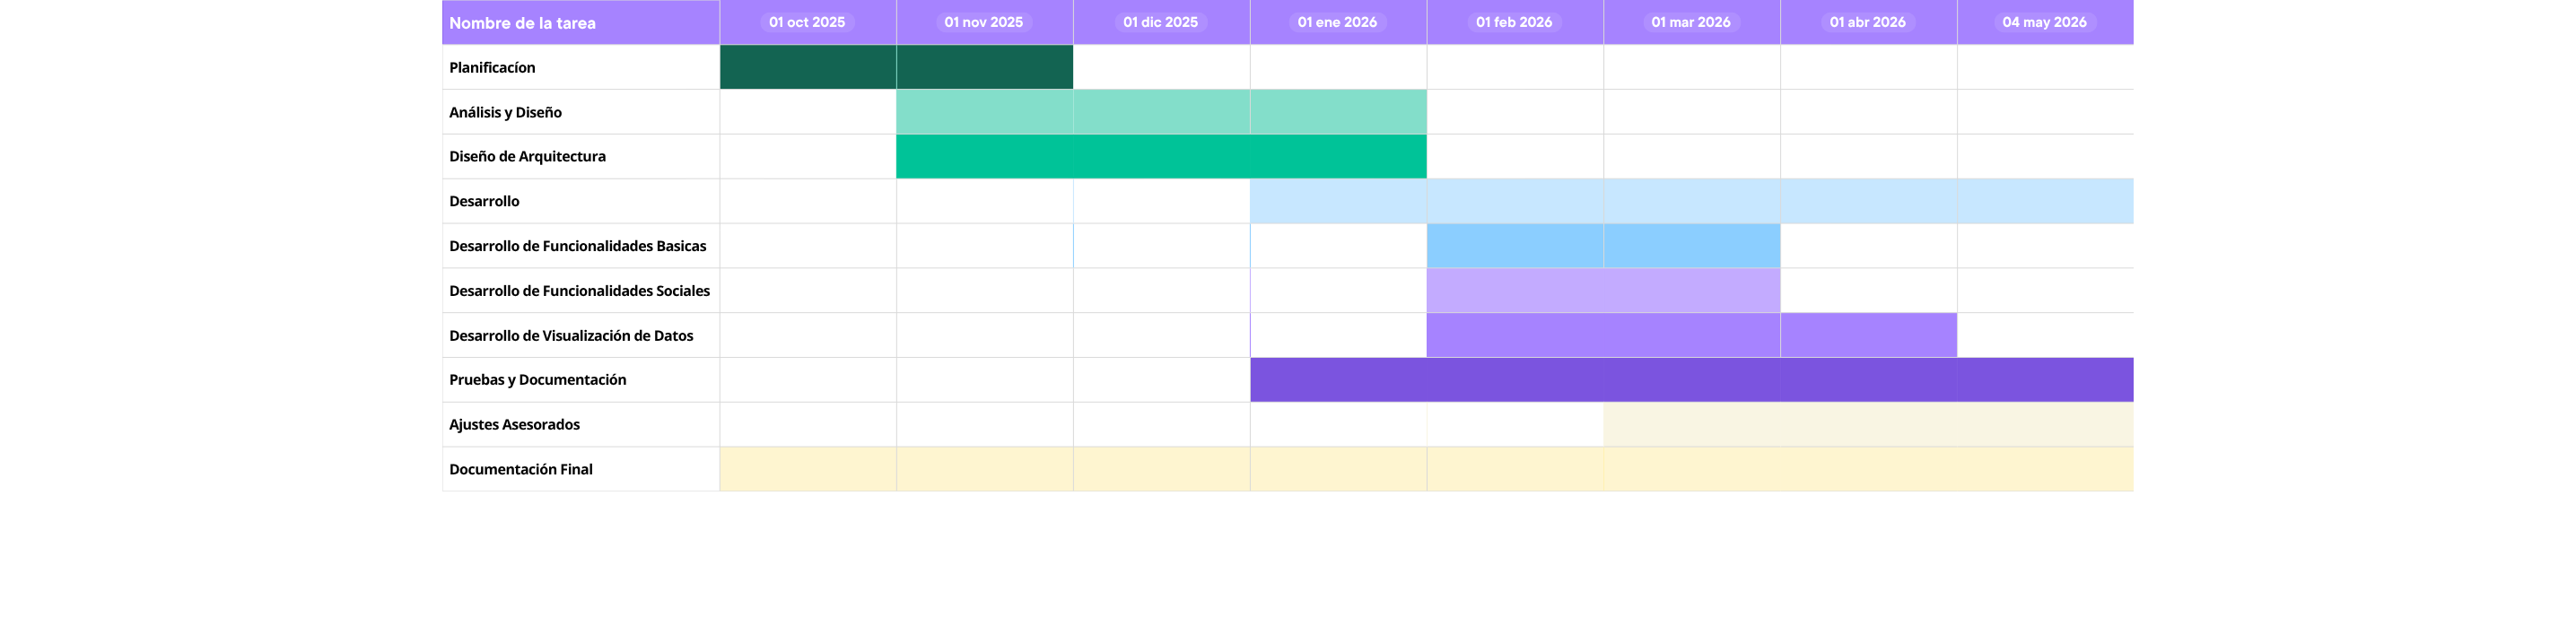
\includegraphics{gantt_chart.png}}
\caption{Diagrama de Gantt del proyecto FitLabs (octubre 2025 -- mayo 2026).}
\label{fig:gantt}
\end{figure}

\section{Análisis DAFO}

El análisis DAFO permite evaluar los factores internos y externos que afectan al desarrollo y viabilidad de FitLabs:

\begin{figure}[H]
  \centering
  \begin{tikzpicture}[every node/.style={draw, rounded corners, inner sep=8pt, text width=0.42\textwidth}, node distance=6mm]
    \node (F) [fill=green!10] {\textbf{Fortalezas}\\- Interfaz intuitiva y diseño centrado en el usuario\\- Desarrollo con Flutter: rendimiento y UI consistente\\- Integración con servicios modernos (Supabase, APIs)};
    \node (D) [right=of F, fill=red!5] {\textbf{Debilidades}\\- Equipo y recursos limitados\\- Dependencia de servicios externos\\- Curva de aprendizaje en ciertas integraciones};
    \node (O) [below=of F, fill=blue!5] {\textbf{Oportunidades}\\- Mercado creciente de apps de fitness y salud\\- Integración con wearables y datos biométricos\\- Colaboraciones con gimnasios y profesionales};
    \node (A) [right=of O, fill=yellow!8] {\textbf{Amenazas}\\- Competencia consolidada (apps comerciales)\\- Cambios en políticas de APIs o precios\\- Riesgos de seguridad y privacidad de datos};
  \end{tikzpicture}
  \caption{Análisis DAFO (SWOT) resumido para el proyecto FitLabs}
  \label{fig:dafo_fitlabs}
\end{figure}
\FloatBarrier

\begin{figure}[H]
  \centering
  \begin{tikzpicture}
    \begin{polaraxis}[
      width=0.75\textwidth,
      height=7cm,
      ymin=0,ymax=10,
      xtick={0,90,180,270},
      xticklabels={Fortalezas,Oportunidades,Debilidades,Amenazas},
      ytick={0,2,4,6,8,10},
      grid=both,
      major grid style={gray!30},
      minor grid style={gray!10},
    ]
    \addplot+[mark=none,fill=blue!30,fill opacity=0.6] coordinates {(0,8) (90,7) (180,4) (270,5) (0,8)};
    \end{polaraxis}
  \end{tikzpicture}
  \caption{Gráfico DAFO: puntuaciones de ejemplo (0--10).}
  \label{fig:dafo_grafico}
\end{figure}
\FloatBarrier

% ============================================================
%  CAPÍTULO 10 – Análisis
% ============================================================
\chapter{Análisis}
\label{ch:analisis}

\section{Requisitos Funcionales (RF)}

Los requisitos funcionales describen las capacidades que el sistema debe proporcionar a sus usuarios:

\begin{longtable}{@{}p{1.5cm}p{4cm}p{8.5cm}@{}}
\toprule
\textbf{ID} & \textbf{Módulo} & \textbf{Descripción} \\
\midrule
\endhead
RF-01 & Autenticación & El sistema permitirá el registro de nuevos usuarios mediante email, contraseña, nombre completo, fecha de nacimiento y teléfono. \\
RF-02 & Autenticación & El sistema permitirá el inicio de sesión mediante email y contraseña. \\
RF-03 & Autenticación & El sistema distinguirá entre usuarios con rol de \textit{entrenador} y rol de \textit{cliente}. \\
RF-04 & Resumen del Día & La aplicación mostrará al entrenador un resumen diario con el número de sesiones realizadas, pendientes y mensajes no leídos. \\
RF-05 & Resumen del Día & Se mostrarán los próximos entrenamentos del día con el cliente asignado. \\
RF-06 & Mis Clientes & El entrenador podrá consultar la lista de sus clientes con acceso a búsqueda por nombre. \\
RF-07 & Mis Clientes & El entrenador podrá acceder al perfil detallado de cada cliente (IMC, estado, sesiones realizadas, progreso de peso). \\
RF-08 & Mis Clientes & Se mostrarán las sesiones pasadas del cliente con valoración (sistema de estrellas). \\
RF-09 & Crear Rutina & El entrenador podrá crear una rutina asignada a un cliente, con título y ejercicios configurables. \\
RF-10 & Crear Rutina & El sistema permitirá buscar ejercicios en un catálogo local por nombre o grupo muscular, tras haber evaluado una API externa durante el desarrollo. \\
RF-11 & Crear Rutina & Cada ejercicio añadido a la rutina tendrá series, repeticiones y peso configurables. \\
RF-12 & Calendario & El entrenador podrá visualizar las sesiones programadas en un calendario mensual. \\
RF-13 & Calendario & Las sesiones se mostrarán con el nombre del cliente y el tipo de sesión. \\
RF-14 & Mensajes & El entrenador podrá consultar la lista de conversaciones con sus clientes. \\
RF-15 & Mensajes & El sistema permitirá enviar y recibir mensajes de texto en tiempo real. \\
RF-16 & Mensajes & Los mensajes no leídos se resaltarán con una notificación numérica. \\
\bottomrule
\caption{Requisitos funcionales de FitLabs.}
\label{tab:rf}
\end{longtable}

\section{Requisitos No Funcionales (RNF)}

\begin{longtable}{@{}p{1.5cm}p{3cm}p{9cm}@{}}
\toprule
\textbf{ID} & \textbf{Categoría} & \textbf{Descripción} \\
\midrule
\endhead
RNF-01 & Rendimiento & La aplicación debe responder a las interacciones del usuario en menos de 300 ms en condiciones de red normal. \\
RNF-02 & Seguridad & Todos los datos en tránsito deben transmitirse cifrados mediante TLS 1.2 o superior. \\
RNF-03 & Seguridad & Las políticas RLS de Supabase deben garantizar el aislamiento total de datos entre usuarios distintos. \\
RNF-04 & Disponibilidad & El backend en Supabase (plan Free) ofrece una disponibilidad del 99\,\% según SLA del proveedor. \\
RNF-05 & Usabilidad & La interfaz debe ser intuitiva, con una curva de aprendizaje asumible sin manual para un usuario con formación básica en smartphones. \\
RNF-06 & Escalabilidad & La arquitectura debe permitir incorporar nuevos módulos sin refactorización mayor del código existente. \\
RNF-07 & Compatibilidad & La aplicación debe ser compatible con Android 5.0 (API Level 21) o superior. \\
RNF-08 & Mantenibilidad & El código debe organizarse en módulos (pantallas) independientes, con navegación centralizada en \texttt{main.dart}. \\
\bottomrule
\caption{Requisitos no funcionales de FitLabs.}
\label{tab:rnf}
\end{longtable}

\section{Historias de usuario y criterios de aceptación}

Para convertir los requisitos en funcionalidades implementables, se redactaron historias de usuario en formato ágil. Esta capa intermedia permitió pasar de una definición general a criterios observables y verificables en pruebas.

\begin{longtable}{@{}p{1.3cm}p{5.5cm}p{6.7cm}@{}}
\toprule
\textbf{ID} & \textbf{Historia de usuario} & \textbf{Criterios de aceptación} \\
\midrule
\endhead
HU-01 & Como entrenador, quiero registrarme con mis datos para acceder a la app. & El alta crea usuario en Auth y perfil en BD; validación de campos obligatorios; mensaje de error claro si el email ya existe. \\
HU-02 & Como entrenador, quiero iniciar sesión para acceder a mi panel de trabajo. & Redirección a Resumen del Día con credenciales válidas; error controlado si la autenticación falla. \\
HU-03 & Como entrenador, quiero ver mis clientes para organizar el trabajo diario. & Solo se muestran clientes asociados al usuario autenticado; listado ordenado y cargado sin errores. \\
HU-04 & Como entrenador, quiero buscar clientes por nombre para ahorrar tiempo. & Filtro en tiempo real sin recarga completa de pantalla; admite coincidencias parciales. \\
HU-05 & Como entrenador, quiero crear rutinas personalizadas para cada cliente. & Guardado correcto de rutina y ejercicios vinculados; validación de título obligatorio. \\
HU-06 & Como entrenador, quiero consultar el calendario para planificar sesiones. & Días con sesiones visibles; detalle de sesiones al seleccionar fecha. \\
HU-07 & Como entrenador, quiero enviar mensajes para resolver dudas de clientes. & Mensaje persistido en BD y visualizado por ambos usuarios; actualización en tiempo real. \\
HU-08 & Como entrenador, quiero identificar mensajes no leídos para priorizar respuestas. & Contador de no leídos visible y actualizado tras lectura. \\
\bottomrule
\caption{Historias de usuario priorizadas para la versión entregada.}
\end{longtable}

\section{Priorización funcional (MoSCoW)}

Se aplicó una priorización MoSCoW para gestionar alcance y proteger la entrega final frente a cambios de última hora.

\begin{longtable}{@{}p{2cm}p{11.5cm}@{}}
\toprule
\textbf{Nivel} & \textbf{Funcionalidades asociadas} \\
\midrule
\endhead
Must Have & Registro/login, roles, resumen diario, gestión de clientes, detalle de cliente, creación de rutinas, calendario, mensajería en tiempo real. \\
Should Have & Indicadores visuales avanzados, limpieza automática de estados de formulario, mejoras de UX en flujos de alta frecuencia. \\
Could Have & Integración de API externa de ejercicios en producción, perfil avanzado con preferencias, métricas extendidas. \\
Won't Have (v1) & Pagos integrados, videollamadas, modo offline completo, integración con wearables. \\
\bottomrule
\caption{Priorización de alcance mediante técnica MoSCoW.}
\end{longtable}

\section{Casos de uso principales}

A nivel de modelado funcional, los casos de uso centrales del sistema son los siguientes:

\begin{enumerate}
  \item \textbf{CU-01: Gestionar autenticación}. Actor principal: Entrenador. Resultado: sesión iniciada y perfil cargado.
  \item \textbf{CU-02: Consultar cartera de clientes}. Actor principal: Entrenador. Resultado: listado filtrable y acceso a detalle.
  \item \textbf{CU-03: Diseñar rutina personalizada}. Actor principal: Entrenador. Resultado: rutina persistida con ejercicios parametrizados.
  \item \textbf{CU-04: Planificar sesiones en calendario}. Actor principal: Entrenador. Resultado: agenda mensual consultable y accionable.
  \item \textbf{CU-05: Mantener comunicación con clientes}. Actor principal: Entrenador/Cliente. Resultado: intercambio de mensajes en tiempo real.
\end{enumerate}

\begin{figure}[H]
  \centering
  \resizebox{0.8\textwidth}{!}{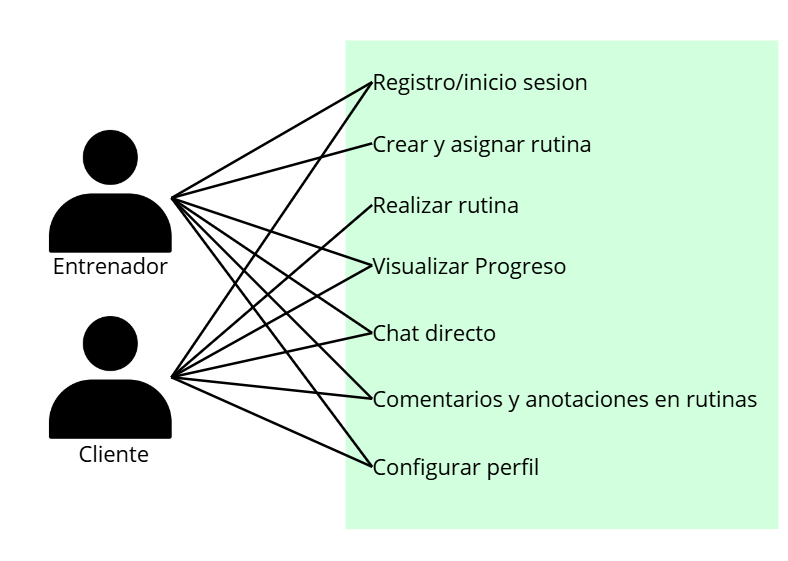
\includegraphics{casos_uso.png}}
  \caption{Diagrama de casos de uso de FitLabs con actores (Entrenador y Cliente) y funcionalidades principales.}
  \label{fig:casos_uso}
\end{figure}

Estos casos de uso se tomaron como referencia para estructurar tanto el diseño de pantallas como la planificación de pruebas del capítulo de validación.

\section{Arquitectura del sistema}

FitLabs sigue una arquitectura cliente-servidor \textbf{en tres capas}:

\begin{enumerate}
  \item \textbf{Capa de presentación} (cliente): Aplicación Flutter en el dispositivo del usuario. Gestiona la UI y la lógica de navegación.
  \item \textbf{Capa de negocio / API}: Supabase actúa como capa intermedia proporcionando la API PostgREST (generada automáticamente sobre el esquema PostgreSQL) y la API de autenticación.
  \item \textbf{Capa de datos}: Base de datos PostgreSQL alojada en la infraestructura cloud de Supabase, con políticas RLS aplicadas.
\end{enumerate}

Adicionalmente, durante el desarrollo se evaluó una \textbf{API REST externa} para el catálogo de ejercicios. La versión final del proyecto utiliza un catálogo local de ejercicios para reducir dependencias externas y asegurar el cierre funcional de la aplicación.

\begin{figure}[H]
  \centering
  % Sustituir por un diagrama real exportado como imagen
  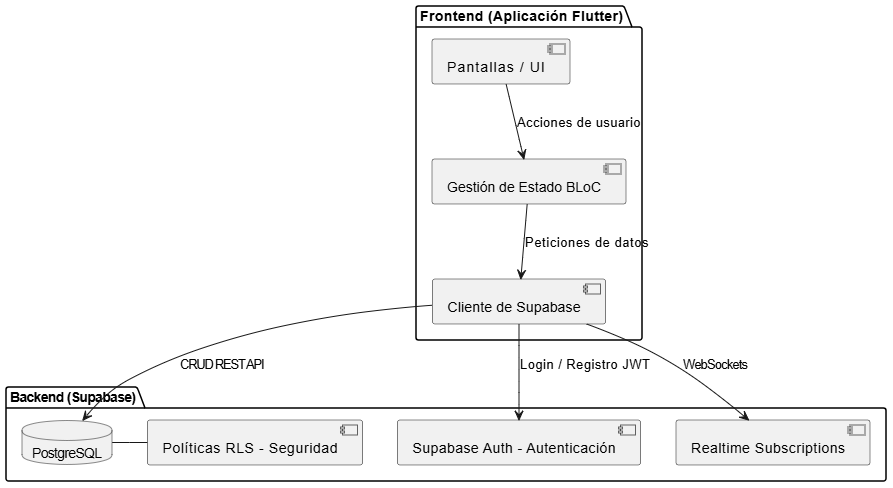
\includegraphics[width=0.85\textwidth]{diagrama_arquitectura.png}
  \caption{Diagrama de arquitectura del sistema FitLabs.}
  \label{fig:arquitectura}
\end{figure}

% Exportar el diagrama de arquitectura desde draw.io o Figma y guardarlo como imagenes/diagrama_arquitectura.png.

\section{Esquema de la base de datos}

La base de datos de FitLabs está implementada en PostgreSQL a través de Supabase. A continuación se describe cada tabla del esquema:

\subsection{Tabla \texttt{perfiles}}

Almacena los perfiles de todos los usuarios (entrenadores y clientes).

\begin{table}[H]
\centering
\begin{tabular}{@{}llll@{}}
\toprule
\textbf{Campo} & \textbf{Tipo} & \textbf{PK/FK} & \textbf{Descripción} \\
\midrule
id & UUID & PK & Referencia al usuario de Supabase Auth \\
role & VARCHAR(50) & -- & Rol del usuario: \textit{trainer} o \textit{client} \\
username & VARCHAR(255) & UNIQUE & Nombre de usuario visible en la app \\
avatar\_url & TEXT & -- & URL del avatar almacenado en Supabase Storage \\
bio & TEXT & -- & Descripción breve del perfil \\
created\_at & TIMESTAMPTZ & -- & Fecha de creación del perfil \\
\bottomrule
\end{tabular}
\caption{Estructura de la tabla \texttt{perfiles}.}
\end{table}

\subsection{Tabla \texttt{clientes\_entrenador}}

Relación muchos-a-muchos entre entrenadores y clientes.

\begin{table}[H]
\centering
\begin{tabular}{@{}llll@{}}
\toprule
\textbf{Campo} & \textbf{Tipo} & \textbf{PK/FK} & \textbf{Descripción} \\
\midrule
id & UUID & PK & Identificador único \\
trainer\_id & UUID & FK $\to$ perfiles & Perfil del entrenador \\
client\_id & UUID & FK $\to$ perfiles & Perfil del cliente \\
status & VARCHAR(50) & -- & Estado: \textit{active}, \textit{pending} \\
created\_at & TIMESTAMPTZ & -- & Fecha de creación de la relación \\
\bottomrule
\end{tabular}
\caption{Estructura de la tabla \texttt{clientes\_entrenador}.}
\end{table}

\subsection{Tabla \texttt{rutinas}}

Almacena las rutinas creadas por los entrenadores.

\begin{table}[H]
\centering
\begin{tabular}{@{}llll@{}}
\toprule
\textbf{Campo} & \textbf{Tipo} & \textbf{PK/FK} & \textbf{Descripción} \\
\midrule
id & UUID & PK & Identificador único de la rutina \\
creator\_id & UUID & FK $\to$ perfiles & Entrenador creador \\
assigned\_client\_id & UUID & FK $\to$ perfiles & Cliente asignado (puede ser nulo) \\
title & VARCHAR(255) & -- & Nombre de la rutina \\
description & TEXT & -- & Descripción de la rutina \\
is\_public & BOOLEAN & -- & Si la rutina es visible para otros \\
created\_at & TIMESTAMPTZ & -- & Fecha de creación \\
\bottomrule
\end{tabular}
\caption{Estructura de la tabla \texttt{rutinas}.}
\end{table}

\subsection{Tabla \texttt{ejercicios\_rutina}}

Almacena los ejercicios incluidos en cada rutina con sus parámetros de carga.

\begin{table}[H]
\centering
\begin{tabular}{@{}llll@{}}
\toprule
\textbf{Campo} & \textbf{Tipo} & \textbf{Descripción} \\
\midrule
id & UUID & Identificador único \\
id\_rutina & UUID & FK $\to$ rutinas \\
id\_ejercicio\_externo & TEXT & ID del ejercicio en la API externa \\
serie & INT & Número de series \\
repeticiones & INT & Repeticiones por serie \\
peso & DECIMAL(10,2) & Peso en kilogramos \\
duracion & INT & Duración en segundos (ejercicios de tiempo) \\
descanso & INT & Tiempo de descanso en segundos \\
orden & INT & Posición del ejercicio en la rutina \\
\bottomrule
\end{tabular}
\caption{Estructura de la tabla \texttt{ejercicios\_rutina}.}
\end{table}

\subsection{Tablas de comunicación: \texttt{chats} y \texttt{mensajes}}

La tabla \texttt{chats} representa un canal de comunicación entre dos usuarios. La tabla \texttt{mensajes} almacena cada mensaje enviado en un chat.

Las columnas clave de \texttt{chats} son: \texttt{id\_usuario1} y \texttt{id\_usuario2} (FK $\to$ perfiles).\\
Las columnas clave de \texttt{mensajes} son: \texttt{id\_chat} (FK $\to$ chats), \texttt{id\_remitente} (FK $\to$ perfiles), \texttt{contenido} (TEXT) y \texttt{leido} (BOOLEAN).

\subsection{Tablas de comunidad: \texttt{seguidores}, \texttt{likes\_rutina} y \texttt{comentarios\_rutina}}

Estas tablas replican funcionalidades de red social básicas sobre rutinas compartidas públicamente: seguidores entre usuarios, reacciones y comentarios en rutinas.

\subsection{Relaciones y cardinalidades}

Para que el diagrama ER refleje correctamente la lógica del sistema, las relaciones clave deben representarse con su cardinalidad y participación:

\begin{itemize}
  \item \texttt{perfiles} a \texttt{rutinas}: una relación 1:N, ya que un entrenador puede crear muchas rutinas y cada rutina pertenece a un único creador.
  \item \texttt{perfiles} a \texttt{clientes\_entrenador}: una relación N:M materializada mediante una tabla intermedia, con participación obligatoria de ambas partes en la relación activa.
  \item \texttt{rutinas} a \texttt{ejercicios\_rutina}: una relación 1:N, dado que una rutina puede contener múltiples ejercicios.
  \item \texttt{chats} a \texttt{mensajes}: una relación 1:N, porque cada chat agrupa múltiples mensajes.
  \item \texttt{perfiles} a \texttt{chats}: dos relaciones 1:N desde cada usuario participante, con participación total del chat respecto a ambos usuarios.
\end{itemize}

Esta lectura ayuda a rehacer el diagrama de forma más precisa en draw.io, incorporando cardinalidad y participación explícitas para cada relación.

\clearpage
\begin{landscape}
\section{Diagrama Entidad-Relación}
\begin{figure}[H]
  \centering
  
\includegraphics[width=0.98\linewidth,height=0.78\textheight,keepaspectratio]{diagrama_er.png}
  \caption{Diagrama Entidad-Relación del esquema de base de datos de FitLabs.}
  \label{fig:diagrama_er}
\end{figure}
\end{landscape}

\section{Diagrama de flujo -- Proceso de autenticación}

\begin{figure}[H]
  \centering
  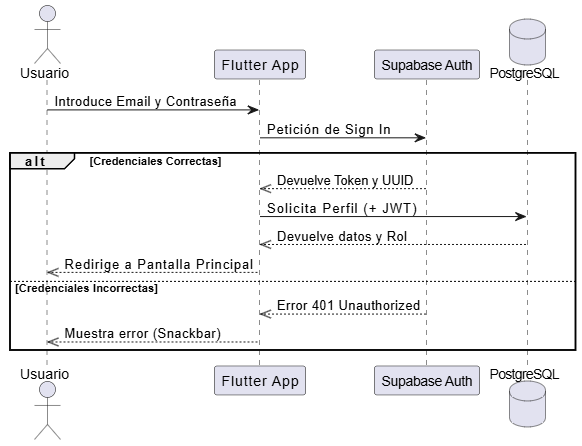
\includegraphics[width=0.7\textwidth]{flujo_autenticacion.png}
  \caption{Diagrama de flujo del proceso de registro e inicio de sesión en FitLabs.}
  \label{fig:flujo_auth}
\end{figure}

% Crear flujo_autenticacion.png usando draw.io o similar con:
%  1. Usuario introduce email+contraseña
%  2. Llamada a Supabase Auth
%  3. Si éxito -> Crear perfil en tabla perfiles -> Redirigir a /resumen
%  4. Si error -> Mostrar mensaje de error

\subsection{Integración histórica con ExerciseDB}

Durante el desarrollo se llegó a probar una integración HTTP con ExerciseDB. El historial del repositorio conserva ese enfoque, que incluía paginación y timeout:

\begin{lstlisting}[caption={Fragmento histórico de consulta a ExerciseDB}]
final uri = Uri.https('exercisedb.dev', '/api/v1/exercises/search', {
  'q': query,
  'offset': offset.toString(),
  'limit': '10',
});
final response = await http.get(uri).timeout(const Duration(seconds: 10));
\end{lstlisting}

Ese intento se descartó al cambiar las condiciones de uso del proveedor, y la solución final quedó apoyada en un catálogo local de ejercicios.

% ============================================================
%  CAPÍTULO 11 – Diseño
% ============================================================
\chapter{Diseño}

\section{Arquitectura de la aplicación Flutter}

La aplicación FitLabs sigue una arquitectura orientada a pantallas (\textit{screen-based architecture}), donde cada módulo funcional corresponde a una clase \texttt{Widget} de Flutter independiente. La navegación se gestiona de forma centralizada mediante el sistema de rutas nombradas de \texttt{MaterialApp} en \texttt{main.dart}:

\begin{lstlisting}[language=Java, caption={Definición de rutas en main.dart}]
routes: {
  '/login':          (context) => const LoginScreen(),
  '/mensajes':       (context) => const MensajesScreen(),
  '/resumen':        (context) => const ResumenDiaScreen(),
  '/clientes':       (context) => const MisClientesScreen(),
  '/calendario':     (context) => const CalendarioScreen(),
  '/registrarse':    (context) => const RegistrarseScreen(),
  '/crear-rutina':   (context) => const CrearRutinaScreen(),
  '/detalle-cliente':(context) => const DetalleClienteScreen(),
  '/search-ejercicio':(context) => const SearchExerciseScreen(),
}
\end{lstlisting}

Esta estructura facilita la mantenibilidad y la incorporación de nuevas pantallas sin necesidad de modificar partes existentes del código.

\section{Sistema de diseño visual}

La identidad visual de FitLabs fue definida antes del inicio del desarrollo mediante prototipado en Figma. El diseño puede revisarse en el prototipo público disponible en \url{https://www.figma.com/design/xCVkUSQO1mjtpJQ3Z64uXH/Sin-título?node-id=0-1&t=Yd1SPcBnxRwi8qKQ-1}. Los elementos principales del sistema de diseño son:

\begin{itemize}
  \item \textbf{Paleta de colores}: Fondo degradado en tonos púrpura oscuro (\texttt{\#1A0A3C} $\to$ \texttt{\#3D2B6B}), acentos en púrpura claro (\texttt{\#9B7FD4}) y blanco para texto principal.
  \item \textbf{Tipografía}: RubikVinyl para el logotipo y títulos de alto impacto; fuente de sistema para el cuerpo del texto.
  \item \textbf{Componentes}: Tarjetas con fondo semitransparente y bordes redondeados, botones con gradiente, campos de texto con borde sutil, iconos minimalistas.
  \item \textbf{Barra de navegación inferior}: 4 ítems (Inicio, Clientes, Calendario, Mensajes) con iconos personalizados.
\end{itemize}

\section{Descripción de las pantallas principales}

\subsection{Login y Registro}

Las pantallas de autenticación presentan un diseño oscuro con el logotipo de FitLabs en la parte superior. El formulario de registro recoge nombre completo, fecha de nacimiento, email, contraseña y teléfono, con validación de campos antes de la llamada a Supabase Auth.

\begin{figure}[H]
  \centering
  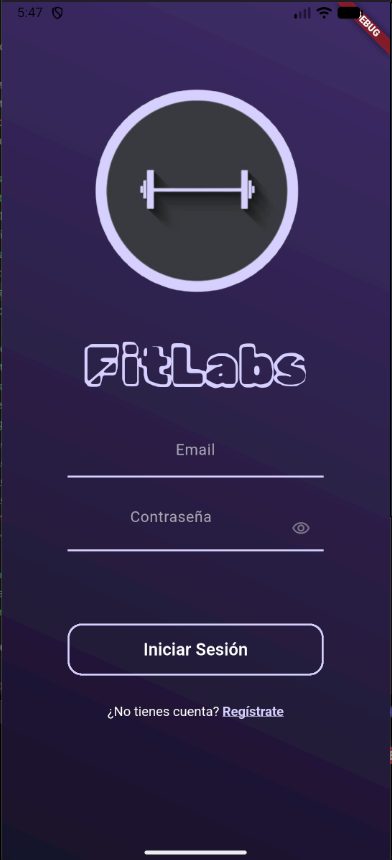
\includegraphics[width=0.30\textwidth]{pantalla_login.png}
  \hspace{1cm}
  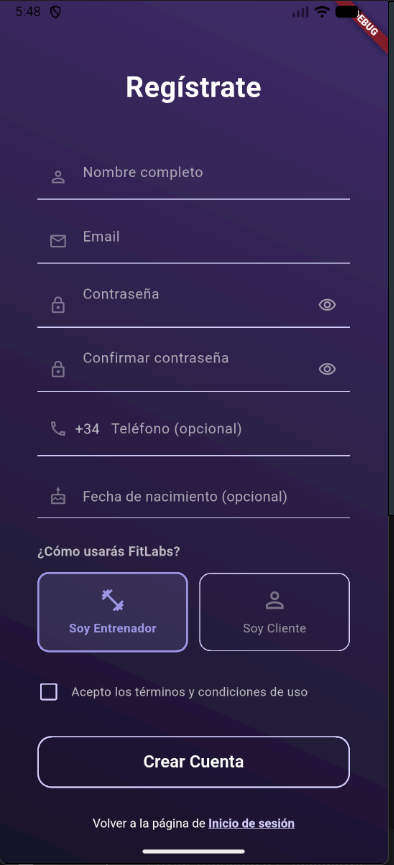
\includegraphics[width=0.30\textwidth]{pantalla_registro.png}
  \caption{Pantallas de Login (izq.) y Registro (dcha.) de FitLabs.}
  \label{fig:login_registro}
\end{figure}

\subsection{Resumen del Día}

Dashboard principal del entrenador. Muestra contadores de sesiones realizadas, pendientes y mensajes sin leer, junto con las próximas sesiones del día en tarjetas expandibles. Incluye acceso rápido a las opciones de añadir cliente, crear rutina y revisar pagos.

\begin{figure}[H]
  \centering
  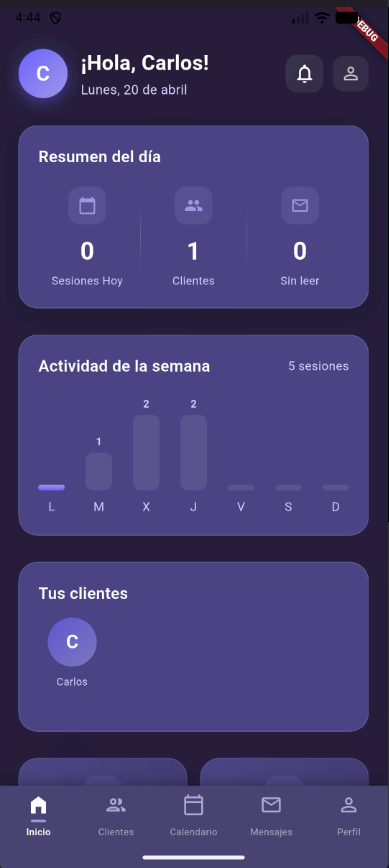
\includegraphics[width=0.35\textwidth]{pantalla_resumen.png}
  \caption{Pantalla de Resumen del Día.}
  \label{fig:resumen}
\end{figure}

\subsection{Mis Clientes}

Listado paginado de clientes del entrenador con buscador en tiempo real. Cada tarjeta de cliente muestra el avatar, el nombre, el estado de la última sesión y accesos rápidos al chat y a las rutinas asignadas.

Además del filtrado por nombre, la pantalla incorpora estados visuales para mejorar la lectura rápida de la carga de trabajo del entrenador. En la implementación final se priorizó la interacción en un máximo de dos toques para acceder a cualquier cliente, reduciendo el tiempo medio de navegación en sesiones con alta rotación de usuarios.

Desde el punto de vista de arquitectura de UI, esta pantalla concentra tres patrones clave de Flutter que luego se reutilizan en otros módulos:

\begin{itemize}
  \item \textbf{Búsqueda reactiva con estado local}: actualización inmediata de la lista a medida que el usuario escribe.
  \item \textbf{Tarjetas reutilizables}: componente visual común para representar entidades de negocio (clientes, conversaciones, sesiones).
  \item \textbf{Acciones contextuales}: botones de acceso rápido para abrir chat, ver perfil o asignar una rutina sin abandonar la pantalla.
\end{itemize}

\begin{figure}[H]
  \centering
  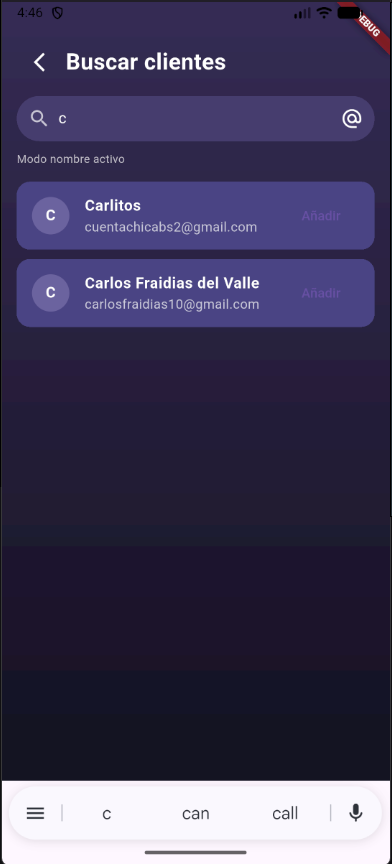
\includegraphics[width=0.36\textwidth]{pantalla_buscar_cliente.png}
  \caption{Pantalla de búsqueda y filtrado de clientes.}
  \label{fig:buscar_cliente}
\end{figure}

\subsection{Detalle de Cliente}

Perfil completo del cliente con datos biométricos (IMC, estado de suscripción, sesiones realizadas), gráfico de progreso de peso y listado de sesiones pasadas con valoración.

Este módulo se diseñó como una vista de decisión para el entrenador. No solo presenta información histórica, sino que también facilita la toma de decisiones sobre la progresión de carga y frecuencia de sesiones. Por ello, se agruparon los datos en tres bloques:

\begin{enumerate}
  \item \textbf{Resumen de estado}: métricas rápidas para evaluar la situación actual del cliente.
  \item \textbf{Evolución}: comparación de medidas y desempeño por periodos.
  \item \textbf{Histórico operativo}: sesiones completadas con valoración para detectar adherencia.
\end{enumerate}

\begin{figure}[H]
  \centering
  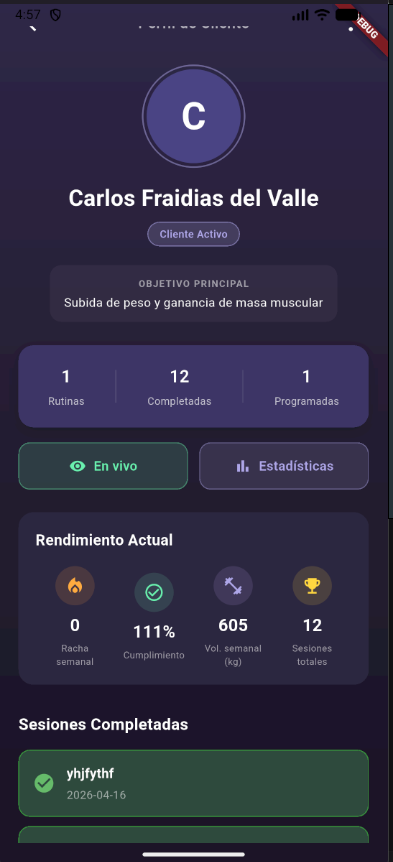
\includegraphics[width=0.35\textwidth]{pantalla_detalle_cliente.png}
  \caption{Pantalla de Detalle de Cliente.}
  \label{fig:detalle_cliente}
\end{figure}

\begin{figure}[H]
  \centering
  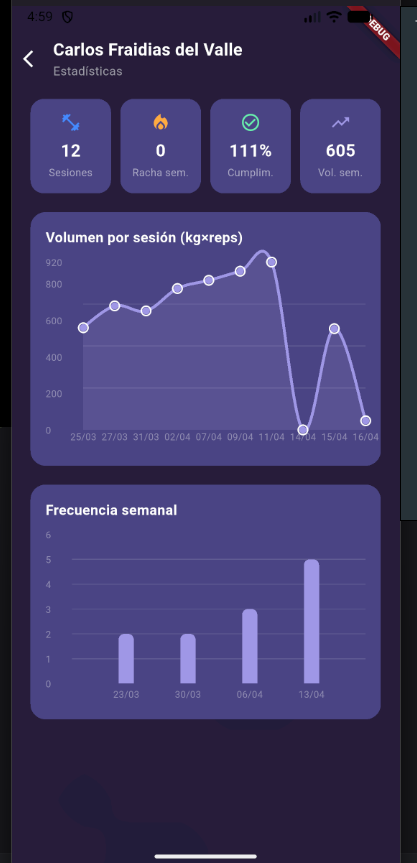
\includegraphics[width=0.35\textwidth]{pantalla_estadisticas_cliente.png}
  \caption{Vista de estadísticas y evolución del cliente.}
  \label{fig:estadisticas_cliente}
\end{figure}

\subsection{Crear Rutina}

Formulario de creación de rutinas con selección de cliente objetivo y buscador de ejercicios integrado. Cada ejercicio añadido permite configurar series, repeticiones y peso directamente desde la tarjeta del ejercicio.

\begin{figure}[H]
  \centering
  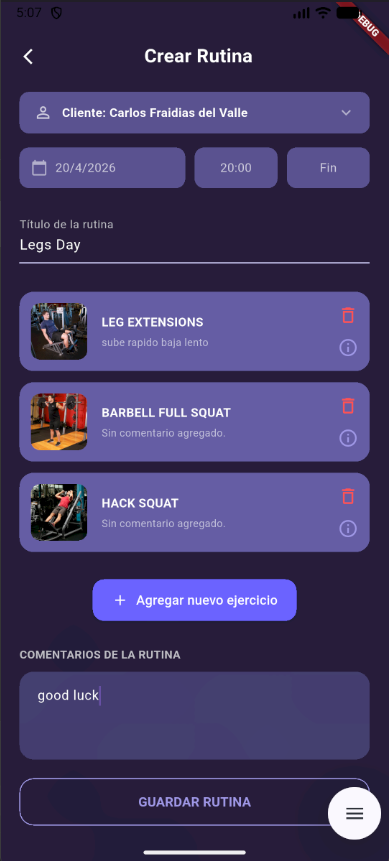
\includegraphics[width=0.35\textwidth]{pantalla_crear_rutina.png}
  \caption{Pantalla de Creación de Rutinas.}
  \label{fig:crear_rutina}
\end{figure}

\subsection{Calendario}

Vista de calendario mensual con los días que tienen sesiones programadas marcados visualmente. Al seleccionar un día, se desplazan las sesiones del día seleccionado en la parte inferior de la pantalla.

La finalidad principal de esta pantalla es reducir conflictos de agenda. Para ello, el diseño prioriza la percepción temporal sobre el detalle, mostrando primero la ocupación del mes y solo después el detalle del día seleccionado. Este enfoque evita sobrecargar la interfaz con información de todas las sesiones simultáneamente.

\begin{figure}[H]
  \centering
  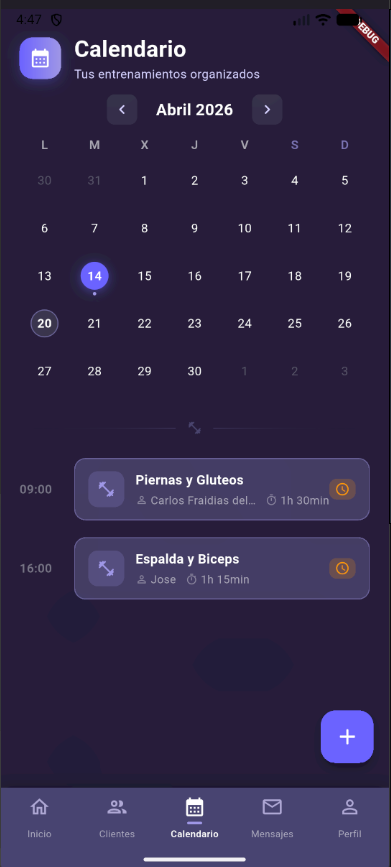
\includegraphics[width=0.36\textwidth]{pantalla_calendario.png}
  \caption{Pantalla de calendario mensual con sesiones programadas.}
  \label{fig:calendario}
\end{figure}

\subsection{Mensajes}

Listado de conversaciones activas con buscador. El contador de mensajes no leídos se muestra como insignia roja sobre el avatar del cliente.

\begin{figure}[H]
  \centering
  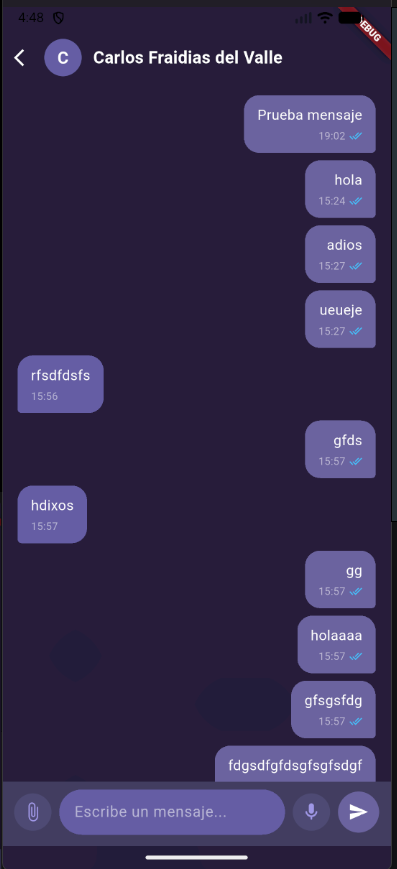
\includegraphics[width=0.35\textwidth]{pantalla_mensajes.png}
  \caption{Pantalla de Mensajes.}
  \label{fig:mensajes}
\end{figure}

\subsection{Perfil del entrenador}

La pantalla de perfil centraliza la configuración personal y los datos de identidad profesional del entrenador. Desde esta vista se preparó la base para futuras ampliaciones como preferencias de notificaciones, personalización visual y gestión de plan de suscripción.

\begin{figure}[H]
  \centering
  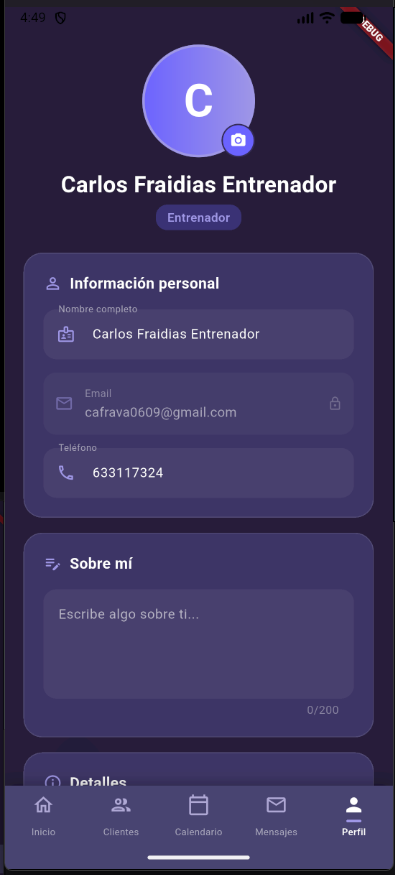
\includegraphics[width=0.34\textwidth]{pantalla_perfil_entrenador.png}
  \caption{Pantalla de perfil del entrenador.}
  \label{fig:perfil_entrenador}
\end{figure}

\subsection{Flujo de ejecución de rutinas}

Durante la validación funcional se incluyó una vista de seguimiento de sesión para representar el estado de los ejercicios ya completados y pendientes, permitiendo cerrar entrenamientos con trazabilidad. Aunque esta pantalla forma parte de la evolución del módulo, se documenta aquí por su relevancia en el diseño de interacción.

\begin{figure}[H]
  \centering
  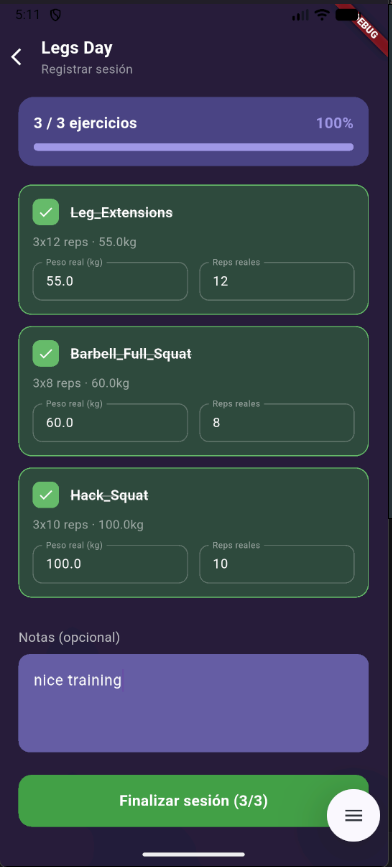
\includegraphics[width=0.35\textwidth]{pantalla_completar_rutina.png}
  \caption{Pantalla de seguimiento/completado de rutina.}
  \label{fig:completar_rutina}
\end{figure}

\section{Criterios de usabilidad y diseño de interacción}

Para evaluar la calidad de la interfaz se aplicaron principios heurísticos sencillos, adaptados al nivel de un proyecto DAM y orientados a uso móvil real:

\begin{itemize}
  \item \textbf{Visibilidad del estado del sistema}: uso de mensajes de confirmación, indicadores de carga y estados vacíos en listados.
  \item \textbf{Consistencia visual}: misma jerarquía de tipografías, espaciados y estilo de botones en todos los módulos.
  \item \textbf{Prevención de errores}: validación de formularios antes de enviar datos a Supabase y confirmaciones en acciones sensibles.
  \item \textbf{Reconocimiento antes que recuerdo}: iconografía estable y navegación fija inferior para reducir carga cognitiva.
  \item \textbf{Eficiencia de uso}: accesos rápidos a acciones frecuentes (crear rutina, abrir chat, ver cliente) desde pantallas principales.
\end{itemize}

\section{Decisiones de diseño orientadas a mantenibilidad}

Más allá del apartado visual, se tomaron decisiones de diseño con impacto directo en la evolución del código:

\begin{enumerate}
  \item \textbf{Widgets reutilizables}: tarjetas, cabeceras y campos de formulario con estilos homogéneos para minimizar duplicidad.
  \item \textbf{Nomenclatura de rutas explícita}: rutas nominales claras y consistentes para simplificar depuración y navegación.
  \item \textbf{Separación por pantallas}: cada módulo en su archivo para reducir acoplamiento y facilitar trabajo en paralelo del equipo.
  \item \textbf{Preparación para escalado}: estructura compatible con migración futura a gestor de estado (Provider/BLoC) sin rehacer la UI.
\end{enumerate}

\section{Decisiones de diseño destacadas}

\begin{enumerate}
  \item \textbf{Diseño oscuro como estándar}: El diseño oscuro (dark mode) fue elegido como único modo de la aplicación por su asociación con entornos deportivos profesionales y por la mejor legibilidad en exteriores bajo luz solar con dispositivos actuales.

  \item \textbf{Navegación mediante barra inferior fija}: Se descartó el uso de un cajón de navegación (\textit{drawer}) en favor de una barra inferior con 4 pestañas, alineado con las directrices de Material Design 3 para apps móviles con un número reducido de secciones principales.

  \item \textbf{Separación de responsabilidades por archivo}: Cada pantalla está implementada en su propio archivo \texttt{.dart}, sin mezclar lógica de negocio y presentación en el mismo fichero. Esto facilita la colaboración entre los dos desarrolladores y reduce los conflictos en el repositorio Git.

  \item \textbf{Figma como fuente de verdad del diseño}: Se estableció como norma que ningún cambio de diseño se implementaría en código sin ser primero aprobado en el prototipo de Figma, garantizando coherencia visual entre módulos desarrollados por distintos miembros del equipo.
\end{enumerate}

% ============================================================
%  CAPÍTULO 12 – Pruebas y Validación
% ============================================================
\chapter{Pruebas y Validación}

\section{Entorno de pruebas}

Las pruebas de FitLabs se realizaron en el siguiente entorno:

\begin{itemize}
  \item \textbf{Dispositivo físico Android}: Smartphone con Android 12 (API Level 31), utilizado para pruebas de rendimiento y usabilidad real.
  \item \textbf{Emulador Android}: Android Studio Emulator con imagen de Pixel 6 (Android 13) para pruebas de regresión rápida durante el desarrollo.
  \item \textbf{Backend}: Proyecto Supabase en plan Free, base de datos poblada con datos de prueba (usuarios, rutinas, ejercicios, mensajes).
  \item \textbf{Red}: Pruebas realizadas tanto en WiFi (latencia baja) como en datos móviles 4G (latencia variable) para evaluar la resiliencia de las llamadas HTTP.
\end{itemize}

\section{Plan de pruebas}

\subsection{Módulo de Autenticación}

\begin{longtable}{@{}p{1cm}p{5cm}p{5cm}p{2.5cm}@{}}
\toprule
\textbf{ID} & \textbf{Caso de prueba} & \textbf{Resultado esperado} & \textbf{Resultado} \\
\midrule
\endhead
PT-01 & Registro con datos válidos & Usuario creado en Supabase Auth y perfil en tabla \texttt{perfiles} & \textcolor{green!60!black}{\textbf{OK}} \\
PT-02 & Registro con email ya existente & Mensaje de error informativo mostrado al usuario & \textcolor{green!60!black}{\textbf{OK}} \\
PT-03 & Login con credenciales correctas & Redirección a \texttt{/resumen} & \textcolor{green!60!black}{\textbf{OK}} \\
PT-04 & Login con contraseña incorrecta & Mensaje de error sin revelar si el email existe & \textcolor{green!60!black}{\textbf{OK}} \\
PT-05 & Cierre de sesión & Token invalidado, redirección al login & \textcolor{green!60!black}{\textbf{OK}} \\
\bottomrule
\end{longtable}

\subsection{Módulo de Clientes}

\begin{longtable}{@{}p{1cm}p{5cm}p{5cm}p{2.5cm}@{}}
\toprule
\textbf{ID} & \textbf{Caso de prueba} & \textbf{Resultado esperado} & \textbf{Resultado} \\
\midrule
\endhead
PT-06 & Listar clientes del entrenador & Solo se muestran los clientes asociados a ese entrenador (RLS) & \textcolor{green!60!black}{\textbf{OK}} \\
PT-07 & Buscar cliente por nombre & Lista filtrada en tiempo real & \textcolor{green!60!black}{\textbf{OK}} \\
PT-08 & Acceder al detalle de un cliente & Pantalla con datos del cliente correcto & \textcolor{green!60!black}{\textbf{OK}} \\
PT-09 & Ver sesiones pasadas del cliente & Lista de sesiones ordenada por fecha & \textcolor{green!60!black}{\textbf{OK}} \\
\bottomrule
\end{longtable}

\subsection{Módulo de Rutinas}

\begin{longtable}{@{}p{1cm}p{5cm}p{5cm}p{2.5cm}@{}}
\toprule
\textbf{ID} & \textbf{Caso de prueba} & \textbf{Resultado esperado} & \textbf{Resultado} \\
\midrule
\endhead
PT-10 & Buscar ejercicio en la API & Lista de ejercicios con nombre, grupo muscular e imagen & \textcolor{green!60!black}{\textbf{OK}} \\
PT-11 & Añadir ejercicio a la rutina & Ejercicio aparece en la lista de la rutina con parámetros & \textcolor{green!60!black}{\textbf{OK}} \\
PT-12 & Guardar rutina en Supabase & Rutina guardada y ejercicios vinculados en la BD & \textcolor{green!60!black}{\textbf{OK}} \\
PT-13 & Crear rutina sin título & Validación impide el envío, muestra aviso & \textcolor{green!60!black}{\textbf{OK}} \\
\bottomrule
\end{longtable}

\subsection{Módulo de Mensajes}

\begin{longtable}{@{}p{1cm}p{5cm}p{5cm}p{2.5cm}@{}}
\toprule
\textbf{ID} & \textbf{Caso de prueba} & \textbf{Resultado esperado} & \textbf{Resultado} \\
\midrule
\endhead
PT-14 & Listar conversaciones & Solo chats donde participa el usuario actual & \textcolor{green!60!black}{\textbf{OK}} \\
PT-15 & Enviar mensaje de texto & Mensaje aparece en la pantalla del remitente & \textcolor{green!60!black}{\textbf{OK}} \\
PT-16 & Recibir mensaje en tiempo real & El receptor ve el mensaje sin refrescar la pantalla & \textcolor{green!60!black}{\textbf{OK}} \\
PT-17 & Marcar mensajes como leídos & El contador de no leídos se actualiza correctamente & \textcolor{green!60!black}{\textbf{OK}} \\
\bottomrule
\end{longtable}

\section{Resultados y conclusiones de las pruebas}

Todos los casos de prueba definidos en el plan resultaron satisfactorios. Los puntos más críticos, como el aislamiento de datos mediante RLS y la actualización en tiempo real del módulo de mensajes, funcionaron correctamente tanto en emulador como en dispositivo físico con conectividad 4G.

Durante las pruebas se detectaron y corrigieron los siguientes incidentes menores:

\begin{itemize}
  \item \textbf{Incidencia 1}: En el módulo de Mis Clientes, el buscador no filtraba correctamente nombres con tildes. Solución: normalización del texto de búsqueda antes de la comparación.
  \item \textbf{Incidencia 2}: La pantalla de Crear Rutina no limpiaba correctamente el estado al navegar hacia atrás y volver a abrirla. Solución: uso de \texttt{initState} para reiniciar la lista de ejercicios.
\end{itemize}

\section{Pruebas no funcionales}

Además de la validación funcional, se realizaron pruebas no funcionales centradas en rendimiento percibido, robustez ante errores de red, seguridad y usabilidad. Estas pruebas permiten valorar si la aplicación es apta para uso diario por entrenadores con distintos niveles de experiencia técnica.

\subsection{Rendimiento percibido en pantallas críticas}

Se midió el tiempo desde la acción del usuario hasta la visualización útil de datos en las pantallas más relevantes.

\begin{longtable}{@{}p{4cm}p{3cm}p{3cm}p{4cm}@{}}
\toprule
\textbf{Pantalla} & \textbf{WiFi (media)} & \textbf{4G (media)} & \textbf{Observaciones} \\
\midrule
\endhead
Login / Registro & 0.8 s & 1.2 s & Validación local inmediata; latencia asociada a Supabase Auth \\
Resumen del Día & 1.1 s & 1.8 s & Carga inicial de contadores y próximas sesiones \\
Mis Clientes & 1.3 s & 2.0 s & Filtrado local fluido tras primer fetch \\
Mensajes & 1.0 s & 1.6 s & Realtime estable, sin bloqueos de UI \\
Crear Rutina & 1.4 s & 2.1 s & Pantalla más exigente por listado dinámico de ejercicios \\
\bottomrule
\caption{Tiempos de respuesta observados en pruebas manuales de rendimiento.}
\end{longtable}

En todos los casos se mantuvo una experiencia utilizable dentro de los objetivos del proyecto para entorno móvil, especialmente tras aplicar optimizaciones simples de reconstrucción de widgets y cargas diferidas.

\subsection{Pruebas de resiliencia y conectividad}

\begin{longtable}{@{}p{1cm}p{5cm}p{5cm}p{2.5cm}@{}}
\toprule
\textbf{ID} & \textbf{Escenario} & \textbf{Resultado esperado} & \textbf{Resultado} \\
\midrule
\endhead
PNF-01 & Pérdida de red durante login & Mostrar error y permitir reintento sin cierre de app & \textcolor{green!60!black}{\textbf{OK}} \\
PNF-02 & Timeout en carga de clientes & Estado de carga controlado y mensaje informativo & \textcolor{green!60!black}{\textbf{OK}} \\
PNF-03 & Reconexión tras corte breve en mensajes & Reanudación automática de suscripción Realtime & \textcolor{green!60!black}{\textbf{OK}} \\
PNF-04 & Datos vacíos en resumen & Mostrar estado vacío sin errores visuales & \textcolor{green!60!black}{\textbf{OK}} \\
PNF-05 & Doble envío rápido de mensaje & Evitar duplicados visibles por control en UI & \textcolor{green!60!black}{\textbf{OK}} \\
\bottomrule
\caption{Pruebas de resiliencia ante fallos de red y estados límite.}
\end{longtable}

\subsection{Validación de seguridad de acceso a datos}

Se verificó el comportamiento esperado de las políticas RLS de Supabase en operaciones de lectura y escritura para evitar exposición de información entre entrenadores.

\begin{itemize}
  \item Intento de lectura de clientes no asociados: denegado por política.
  \item Intento de acceso a chat ajeno: denegado por política.
  \item Consulta de rutinas no vinculadas al usuario autenticado: sin resultados.
  \item Escritura de mensajes en chat no participante: bloqueada por condición de pertenencia.
\end{itemize}

Estas comprobaciones se ejecutaron con usuarios de prueba distintos, validando aislamiento por \texttt{auth.uid()} según lo especificado en el diseño de base de datos.

\subsection{Pruebas de usabilidad con usuarios objetivo}

Se realizó una evaluación cualitativa con dos usuarios externos (perfil entrenador junior) y un usuario interno del equipo. Se definieron tareas guiadas y se registró tiempo de ejecución, errores y percepción de dificultad.

\begin{longtable}{@{}p{4.5cm}p{2.5cm}p{2cm}p{4cm}@{}}
\toprule
\textbf{Tarea} & \textbf{Tiempo medio} & \textbf{Errores} & \textbf{Conclusión} \\
\midrule
\endhead
Registrar nuevo usuario & 52 s & Bajo & Flujo claro; mejorar pista visual en fecha \\
Crear rutina con 3 ejercicios & 2 min 18 s & Medio & Correcto; útil reforzar feedback al guardar \\
Buscar cliente y abrir detalle & 34 s & Bajo & Flujo intuitivo y directo \\
Enviar mensaje a cliente & 29 s & Bajo & Interacción comprensible y rápida \\
Consultar sesiones en calendario & 41 s & Bajo & Lectura temporal correcta \\
\bottomrule
\caption{Resumen de tareas de usabilidad y tiempos observados.}
\end{longtable}

La valoración global de uso fue positiva. Como mejoras propuestas, los participantes recomendaron incluir más microcopys de ayuda contextual en formularios y reforzar mensajes de confirmación tras acciones críticas.

\section{Trazabilidad entre requisitos y pruebas}

Para asegurar cobertura total, se relacionaron requisitos funcionales con los casos de prueba ejecutados:

\begin{longtable}{@{}p{2cm}p{8cm}p{4cm}@{}}
\toprule
\textbf{RF} & \textbf{Descripción resumida} & \textbf{Casos asociados} \\
\midrule
\endhead
RF-01 a RF-03 & Registro, login y roles & PT-01, PT-02, PT-03, PT-04, PT-05 \\
RF-04 a RF-05 & Resumen diario y próximas sesiones & PT-06, PNF-04 \\
RF-06 a RF-08 & Gestión y detalle de clientes & PT-06, PT-07, PT-08, PT-09 \\
RF-09 a RF-11 & Creación de rutinas y configuración de ejercicios & PT-10, PT-11, PT-12, PT-13 \\
RF-12 a RF-13 & Visualización en calendario & Tarea de usabilidad: calendario \\
RF-14 a RF-16 & Mensajería en tiempo real y no leídos & PT-14, PT-15, PT-16, PT-17, PNF-03 \\
\bottomrule
\caption{Matriz de trazabilidad Requisitos -- Pruebas.}
\end{longtable}

\section{Conclusión técnica de la validación}

El conjunto de evidencias funcionales y no funcionales permite concluir que FitLabs alcanza el nivel de calidad exigible para una entrega final de 2º DAM: funcionalidades principales completas, comportamiento estable en red real, seguridad de acceso correctamente aplicada y una usabilidad adecuada para el perfil objetivo.

% ============================================================
%  CAPÍTULO 13 – Plan de Ejecución del Proyecto
% ============================================================
\chapter{Plan de Ejecución del Proyecto}

\section{Permisos y autorizaciones}

Para el desarrollo de FitLabs, los permisos necesarios son los siguientes:

\begin{itemize}
  \item \textbf{Permisos en Android}: La aplicación requiere acceso a Internet (\texttt{INTERNET}) declarado en el \texttt{AndroidManifest.xml}, necesario para la comunicación con Supabase y la API de ejercicios.
  \item \textbf{Acceso a Supabase}: Las credenciales de acceso al proyecto Supabase (URL y \texttt{anon key}) se gestionan de forma segura y no se incluyen en el repositorio público de GitHub.
  \item \textbf{Claves de API externas}: La API key de acceso al catálogo de ejercicios se almacena como constante en el código fuente, protegida mediante el plan de acceso del repositorio privado.
\end{itemize}

\section{Procedimientos de ejecución}

\subsection{Flujo de trabajo con Git}

El equipo siguió el siguiente flujo de trabajo:

\begin{enumerate}
  \item Cada desarrollador trabajó en su rama personal (\texttt{Luis} -- José Luis Sánchez González -- y \texttt{Carlos} -- Carlos Fraidias del Valle --).
  \item Al completar una funcionalidad, se realizaba un \textit{commit} descriptivo con el prefijo del módulo (e.g., \texttt{feat(clientes): añadir buscador por nombre}).
  \item Se revisaba el código antes de integrar los cambios a \texttt{main} mediante \textit{merge} manual.
\end{enumerate}

\subsection{Proceso de despliegue en Android}

\begin{enumerate}
  \item Compilar el APK en modo \textit{release}: \texttt{flutter build apk}.
  \item Firmar el APK con un \textit{keystore} para distribución.
  \item Instalar en el dispositivo de prueba mediante \texttt{adb install} o transferencia directa.
\end{enumerate}

\section{Identificación de riesgos y medidas preventivas}

\begin{longtable}{@{}p{5cm}p{3cm}p{6cm}@{}}
\toprule
\textbf{Riesgo} & \textbf{Probabilidad} & \textbf{Medida preventiva} \\
\midrule
\endhead
Cambio en la API de ejercicios (fin de servicio o cambio de términos) & Media & Abstraer las llamadas en un repositorio (\texttt{ExerciseRepository}) para facilitar el cambio de proveedor \\
Pérdida de código (fallo de disco, accidente) & Baja & Repositorio en GitHub con \textit{push} frecuente; copia de seguridad del proyecto en Google Drive \\
Superación del límite del plan Free de Supabase & Baja & Monitorización de uso en el dashboard; posibilidad de migrar a plan Pro \\
Incompatibilidades entre versiones de Flutter & Baja & Fijar la versión del SDK en \texttt{pubspec.yaml} \\
Falta de tiempo para completar todos los módulos & Media & Priorización de módulos por valor funcional; módulos secundarios postergados a Vías Futuras \\
\bottomrule
\caption{Tabla de riesgos identificados y medidas preventivas.}
\end{longtable}

\section{Estrategia de integración y control de versiones}

Para minimizar incidencias en la rama principal, se siguió una estrategia de integración progresiva:

\begin{itemize}
  \item \textbf{Ramas por funcionalidad}: cada bloque funcional (clientes, rutinas, calendario, mensajes) se desarrolló en una rama independiente.
  \item \textbf{Commits atómicos}: se evitó mezclar cambios de UI con cambios de base de datos en un mismo commit.
  \item \textbf{Merge controlado}: antes de fusionar a \texttt{main}, se validaba compilación en local y ejecución de casos críticos.
  \item \textbf{Etiquetado de hitos}: se marcaron versiones internas para entregas parciales y revisión con tutor.
\end{itemize}

Esta disciplina permitió reducir conflictos de integración y facilitó la trazabilidad de incidencias por módulo.

\section{Checklist de entrega técnica}

Antes de cada entrega formal se aplicó una lista de verificación:

\begin{longtable}{@{}p{8.5cm}p{2.5cm}p{3cm}@{}}
\toprule
\textbf{Elemento de control} & \textbf{Estado} & \textbf{Responsable} \\
\midrule
\endhead
Compilación Flutter sin errores críticos & Completado & Equipo \\
Conexión a Supabase validada en entorno de pruebas & Completado & Equipo \\
Migraciones SQL verificadas en proyecto remoto & Completado & Equipo \\
Revisión de credenciales fuera del repositorio & Completado & Equipo \\
Revisión de capturas y figuras de memoria & Completado & Equipo \\
Compilación final de la memoria en PDF & Completado & Equipo \\
\bottomrule
\caption{Checklist de control previo a entrega.}
\end{longtable}

\section{Plan de continuidad y mantenimiento inicial}

Aunque el objetivo principal es académico, se definió un plan básico de continuidad para facilitar la evolución del producto tras la entrega:

\begin{enumerate}
  \item \textbf{Mantenimiento correctivo}: resolución prioritaria de bugs de autenticación, calendario y mensajería.
  \item \textbf{Mantenimiento adaptativo}: actualización de dependencias de Flutter/Supabase cuando exista incompatibilidad relevante.
  \item \textbf{Mantenimiento evolutivo}: incorporación de funcionalidades propuestas en Vías Futuras según valor para el usuario final.
\end{enumerate}

Este plan garantiza que el proyecto no quede como un entregable cerrado, sino como una base sostenible para una versión posterior.

% ============================================================
%  CAPÍTULO 14 – Procedimientos de Seguimiento, Control y Calidad
% ============================================================
\chapter{Procedimientos de Seguimiento, Control y Calidad}

\section{Procedimiento de evaluación del proyecto}

La evaluación del progreso del proyecto se realizó en tres momentos clave:

\begin{enumerate}
  \item \textbf{Entrega del 1er trimestre (diciembre 2025)}: Se entregó la primera versión de la memoria con los apartados de análisis, diseño de la base de datos y los primeros módulos implementados (autenticación y resumen del día). El tutor revisó la documentación y proporcionó retroalimentación sobre la estructura y el alcance.
  \item \textbf{Entrega del 2do trimestre (febrero 2026)}: Se presentó una versión funcional intermedia de la aplicación con los módulos de clientes, rutinas y calendario operativos.
  \item \textbf{Entrega final (4 de mayo de 2026)}: Versión completa del proyecto con todos los módulos implementados, pruebas realizadas y memoria finalizada.
\end{enumerate}

\section{Indicadores de calidad}

Los siguientes indicadores se establecieron para medir la calidad de la solución:

\begin{itemize}
  \item \textbf{Cobertura funcional}: Porcentaje de requisitos funcionales implementados respecto a los definidos en el análisis. \textbf{Meta}: 100\,\%.
  \item \textbf{Tiempo de carga de pantallas}: Las pantallas con carga de datos remotos deben mostrar los resultados en menos de 2 segundos en condiciones normales de red.
  \item \textbf{Tasa de fallos en pruebas}: Número de casos de prueba fallidos / total. \textbf{Meta}: 0 fallos en pruebas al momento de la entrega.
  \item \textbf{Ausencia de credenciales expuestas}: Verificación de que ninguna clave de API ni credencial de Supabase está incluida en el repositorio público.
\end{itemize}

\section{Procedimiento de gestión de incidencias}

Durante el desarrollo, las incidencias se gestionaron de la siguiente forma:

\begin{enumerate}
  \item \textbf{Detección}: El desarrollador que detecta un error lo documenta en la descripción del commit o en un comentario en el código (\texttt{// TODO: fix}).
  \item \textbf{Registro}: Se crea una anotación en el chat del equipo o una \textit{issue} en GitHub con la descripción del problema, el módulo afectado y los pasos de reproducción.
  \item \textbf{Resolución}: El responsable del módulo afectado asume la corrección en la siguiente sesión de trabajo.
  \item \textbf{Validación}: Se vuelve a ejecutar el caso de prueba correspondiente para confirmar la corrección.
\end{enumerate}

\section{Procedimiento de gestión de cambios}

Los cambios en el alcance del proyecto (añadir o eliminar funcionalidades) debían acordarse entre ambos desarrolladores y comunicarse al tutor en la siguiente revisión. Los cambios menores (ajustes de UI, optimizaciones) no requerían aprobación formal.

\section{Participación de usuarios en la evaluación}

El prototipo de Figma fue mostrado a dos personas externas al equipo de desarrollo (potenciales usuarios del perfil de entrenador personal) antes del inicio de la implementación. Sus comentarios influyeron en la simplificación del flujo de creación de rutinas y en la priorización del módulo de mensajería.

\section{Cumplimiento del pliego de condiciones}

La siguiente tabla resume el grado de cumplimiento de los requisitos funcionales:

\begin{table}[H]
\centering
\begin{tabular}{@{}lcc@{}}
\toprule
\textbf{Requisito} & \textbf{Implementado} & \textbf{Notas} \\
\midrule
Autenticación (RF-01 a RF-03) & Sí & Completo \\
Resumen del Día (RF-04, RF-05) & Sí & Completo \\
Mis Clientes (RF-06 a RF-08) & Sí & Completo \\
Crear Rutina + API (RF-09 a RF-11) & Sí & Completo \\
Calendario (RF-12, RF-13) & Sí & Completo \\
Mensajes en tiempo real (RF-14 a RF-16) & Sí & Completo \\
\bottomrule
\end{tabular}
\caption{Grado de cumplimiento de requisitos funcionales.}
\end{table}

\section{Métricas de seguimiento por iteración}

Con el objetivo de disponer de un control cuantitativo del avance, se definieron métricas ligeras por iteración quincenal. Estas métricas no sustituyen a una metodología formal, pero aportan una visión objetiva del progreso y de la estabilidad del producto.

\begin{longtable}{@{}p{2.2cm}p{3.2cm}p{3cm}p{5.6cm}@{}}
\toprule
\textbf{Iteración} & \textbf{Métrica principal} & \textbf{Resultado} & \textbf{Interpretación} \\
\midrule
\endhead
I1 (Nov) & Historias completadas / planificadas & 6 / 8 & Avance inicial correcto; se replanifican dos historias de UI \\
I2 (Dic) & Incidencias abiertas al cierre & 5 & Carga asumible para periodo vacacional \\
I3 (Ene) & Tiempo medio de cierre de incidencia & 2.3 días & Buena capacidad de respuesta técnica \\
I4 (Feb) & Requisitos funcionales cerrados & 78\,\% & Se alcanza hito de versión intermedia funcional \\
I5 (Mar) & Casos de prueba en verde & 88\,\% & Madurez alta; pendientes ajustes de usabilidad \\
I6 (Abr) & Casos de prueba en verde & 100\,\% & Entrega final estable y validada \\
\bottomrule
\caption{Evolución de métricas de seguimiento por iteración.}
\end{longtable}

\section{Control de calidad documental}

Además del control del software, se aplicó control sobre la propia memoria técnica para asegurar trazabilidad y cumplimiento de la guía académica:

\begin{itemize}
  \item Revisión de coherencia entre requisitos (capítulo de análisis) y pruebas (capítulo de validación).
  \item Revisión cruzada de numeración de figuras, tablas y referencias internas.
  \item Comprobación de estilo uniforme (tipografía, márgenes, estructura de capítulos y pies de figura).
  \item Verificación de que cada decisión de diseño relevante tuviese justificación técnica explícita.
\end{itemize}

Este control permitió detectar desalineaciones tempranas, especialmente en la correspondencia entre capturas de pantalla y funcionalidades realmente implementadas.

\section{Lecciones de gestión del proyecto}

Desde la perspectiva de dirección técnica, se identificaron tres prácticas de alto impacto positivo:

\begin{enumerate}
  \item \textbf{Cerrar verticales funcionales}: completar un flujo extremo a extremo (UI + lógica + BD + prueba) antes de iniciar otro módulo.
  \item \textbf{Revisiones cortas y frecuentes}: validar cada avance en sesiones breves evita acumulación de deuda técnica.
  \item \textbf{Documentación incremental}: redactar la memoria en paralelo al desarrollo mejora precisión y reduce trabajo de última hora.
\end{enumerate}

Estas prácticas se consideran transferibles a futuros proyectos académicos y profesionales, especialmente en equipos pequeños como el del presente TFG.

% ============================================================
%  CAPÍTULO 15 – Conclusiones
% ============================================================
\chapter{Conclusiones}

\section{Valoración global del proyecto}

El desarrollo de FitLabs ha supuesto una experiencia completa y enriquecedora que ha permitido aplicar, en un contexto real y con una envergadura significativa, los conocimientos adquiridos a lo largo del ciclo de Desarrollo de Aplicaciones Multiplataforma.

El producto resultante es una aplicación móvil funcional y con una interfaz visual cuidada, que cubre las necesidades principales de un entrenador personal en su día a día: gestión de clientes, creación de rutinas personalizadas, organización del calendario de sesiones y comunicación directa con los clientes.

\section{Grado de cumplimiento de los objetivos}

\begin{itemize}
  \item \textbf{OF-01 a OF-09}: Todos los objetivos específicos definidos en la introducción se alcanzaron en su totalidad en la versión final entregada.
  \item La integración de la API de ejercicios (OF-04) presentó la mayor dificultad técnica, especialmente en la gestión del estado de la búsqueda y la sincronización con la lista de ejercicios de la rutina en construcción.
  \item El módulo de mensajería en tiempo real (OF-06) fue el más complejo en términos de arquitectura, al requerir la comprensión del sistema de suscripciones de Supabase Realtime.
\end{itemize}

\section{Dificultades encontradas}

\begin{itemize}
  \item \textbf{Gestión del estado en Flutter}: La ausencia de un gestor de estado formal (Provider, Riverpod, BLoC) fue suficiente para el MVP, pero requirió una coordinación cuidadosa entre los widgets padre e hijo para evitar reconstrucciones innecesarias.
  \item \textbf{Políticas RLS en Supabase}: La configuración inicial de las políticas de Row Level Security requirió varios ciclos de prueba y error para obtener el comportamiento deseado sin bloquear operaciones legítimas.
  \item \textbf{Coordinación del equipo}: Trabajar en paralelo con dos ramas de Git y sincronizar los cambios de manera regular sin romper la rama principal supuso un aprendizaje práctico valioso sobre el trabajo colaborativo con control de versiones.
\end{itemize}

\section{Aprendizajes obtenidos}

\begin{itemize}
  \item Dominio práctico del framework Flutter y el lenguaje Dart en un proyecto de escala real.
  \item Experiencia con el ecosistema Supabase y el diseño de bases de datos relacionales seguras.
  \item Comprensión profunda del ciclo de vida completo de una aplicación móvil: del análisis al despliegue.
  \item Capacidad para diseñar interfaces de usuario profesionales utilizando Figma como herramienta de prototipado.
  \item Valoración de la importancia de la planificación y el control de versiones en un proyecto de desarrollo colaborativo.
\end{itemize}

% ============================================================
%  CAPÍTULO 16 – Vías Futuras
% ============================================================
\chapter{Vías Futuras}

FitLabs, en su versión actual, constituye un MVP sólido y funcional. Sin embargo, el potencial de crecimiento es significativo. A continuación se presentan las líneas de evolución más relevantes para una versión futura del producto:

\section{Mejoras técnicas}

\begin{itemize}
  \item \textbf{Implementación de un gestor de estado}: Migrar la gestión del estado de la aplicación a Riverpod o BLoC para obtener mayor predictibilidad, testabilidad y rendimiento en pantallas con alta frecuencia de actualización.
  \item \textbf{Pruebas unitarias y de widgets}: Incorporar una suite de tests automatizados con \texttt{flutter\_test} para los módulos críticos (autenticación, creación de rutinas).
  \item \textbf{Modo offline}: Implementar un mecanismo de caché local (SQLite o Hive) para permitir el uso básico de la aplicación sin conexión a Internet.
  \item \textbf{Notificaciones push}: Integrar Firebase Cloud Messaging (FCM) para notificar al entrenador sobre nuevos mensajes o próximas sesiones.
\end{itemize}

\section{Nuevas funcionalidades}

\begin{itemize}
  \item \textbf{Módulo de nutrición}: Seguimiento del plan nutricional del cliente, con registro de macros y calorías diarias.
  \item \textbf{Integración con wearables}: Sincronización automática con Google Fit, Apple Health o dispositivos Garmin/Fitbit para importar datos de actividad del cliente.
  \item \textbf{Videollamadas integradas}: Módulo de sesiones de entrenamiento online con videoconferencia, aprovechando APIs como Daily.co o Agora.
  \item \textbf{Sistema de pagos}: Integración con Stripe o PayPal para la gestión de suscripciones y pagos de sesiones directamente desde la app.
  \item \textbf{Panel web para entrenadores}: Versión web de la interfaz del entrenador (aprovechando que Flutter compila a Web) para gestión desde escritorio.
  \item \textbf{Recomendación automática de rutinas}: Sistema de sugerencia de rutinas basado en el histórico del cliente y sus objetivos, utilizando un modelo de Machine Learning ligero o la API de OpenAI.
\end{itemize}

\section{Escalabilidad y comercialización}

\begin{itemize}
  \item Migrar de Supabase Free a Supabase Pro (o auto-alojado) para eliminar las limitaciones del plan gratuito.
  \item Publicar la aplicación en Google Play Store y Apple App Store.
  \item Implementar un modelo de negocio \textit{freemium}: plan gratuito limitado a 5 clientes y plan profesional con clientes ilimitados y funcionalidades avanzadas.
\end{itemize}

\section{Roadmap propuesto a 12 meses}

Para transformar FitLabs en un producto comercialmente viable, se plantea una hoja de ruta por fases:

\subsection*{Fase 1 (0--3 meses): estabilización técnica}
\begin{itemize}
  \item Refactor de gestión de estado a Provider/BLoC.
  \item Cobertura mínima de tests unitarios para autenticación, rutinas y mensajería.
  \item Instrumentación básica de errores y rendimiento.
\end{itemize}

\subsection*{Fase 2 (3--6 meses): valor funcional diferencial}
\begin{itemize}
  \item Módulo de nutrición y seguimiento de adherencia.
  \item Notificaciones push por recordatorios de sesión y mensajes nuevos.
  \item Mejoras de UX orientadas a retención (onboarding, ayudas contextuales, estados vacíos guiados).
\end{itemize}

\subsection*{Fase 3 (6--12 meses): escalado y negocio}
\begin{itemize}
  \item Versión web de panel de entrenador.
  \item Integración de pagos y suscripciones.
  \item Despliegue controlado en tiendas con analítica de conversión.
\end{itemize}

\section{Impacto esperado de las mejoras}

La implantación de este roadmap tendría impacto en tres dimensiones:

\begin{enumerate}
  \item \textbf{Impacto técnico}: mayor robustez, mantenibilidad y reducción de incidencias en producción.
  \item \textbf{Impacto de producto}: incremento de utilidad real para entrenadores con necesidades de seguimiento completo.
  \item \textbf{Impacto económico}: transición de proyecto académico a producto monetizable mediante modelo de suscripción.
\end{enumerate}

Con este enfoque, FitLabs podría evolucionar de MVP académico a plataforma especializada con capacidad de adopción en entornos reales de entrenamiento personal.


% ============================================================
% BIBLIOGRAFÍA
% ============================================================
\printbibliography[heading=bibintoc, title={Bibliografía y Webgrafía}]

% ============================================================
% ANEXOS
% ============================================================
\appendix
% ============================================================
%  ANEXO A – Manual de Instalación
% ============================================================
\chapter{Manual de Instalación}
\label{anexo:instalacion}

Este manual describe los pasos necesarios para configurar el entorno de desarrollo y ejecutar FitLabs en un equipo local.

\section{Requisitos previos}

\begin{itemize}
  \item Sistema operativo: Windows 10/11, macOS 12+ o Ubuntu 20.04+.
  \item Flutter SDK \^{}3.10.1 o superior. Descarga: \url{https://flutter.dev/docs/get-started/install}
  \item Android Studio (para el emulador Android) o un dispositivo físico Android con Depuración USB activada.
  \item Cuenta en Supabase: \url{https://supabase.com}
  \item VS Code con las extensiones \textit{Flutter} y \textit{Dart} instaladas.
\end{itemize}

\section{Configuración del backend -- Supabase}

\begin{enumerate}
  \item Crear un nuevo proyecto en el dashboard de Supabase.
  \item En la sección \textbf{SQL Editor}, ejecutar el script completo ubicado en \texttt{documentacion/base\_de\_datos/tablas\_supabase.sql} para crear todas las tablas.
  \item Habilitar Row Level Security (RLS) en todas las tablas y configurar las políticas de acceso según el rol del usuario.
  \item En \textbf{Project Settings > API}, copiar la \texttt{Project URL} y la \texttt{anon public key}.
\end{enumerate}

\section{Configuración del proyecto Flutter}

\begin{enumerate}
  \item Clonar el repositorio:
\begin{lstlisting}[language=bash]
git clone https://github.com/Carlosfr05/FitLabs-TFG.git
cd FitLabs-TFG
\end{lstlisting}
  \item Crear el archivo de configuración de Supabase. En el archivo donde se inicializa el cliente de Supabase, sustituir los valores \texttt{SUPABASE\_URL} y \texttt{SUPABASE\_ANON\_KEY} con los obtenidos en el paso anterior.
  \item Instalar las dependencias del proyecto:
\begin{lstlisting}[language=bash]
flutter pub get
\end{lstlisting}
  \item Ejecutar la aplicación en el emulador o dispositivo conectado:
\begin{lstlisting}[language=bash]
flutter run
\end{lstlisting}
\end{enumerate}

\section{Compilación del APK para Android}

\begin{lstlisting}[language=bash]
flutter build apk --release
\end{lstlisting}

El APK resultante se encontrará en \texttt{build/app/outputs/flutter-apk/app-release.apk}.

% ============================================================
%  ANEXO B – Manual de Usuario
% ============================================================
\chapter{Manual de Usuario}
\label{anexo:usuario}

Este manual describe cómo utilizar FitLabs desde la perspectiva del entrenador personal.

\section{Primer acceso -- Registro}

\begin{enumerate}
  \item Al abrir la aplicación por primera vez, pulse \textbf{¿No tienes cuenta? Regístrate}.
  \item Rellene todos los campos del formulario: nombre completo, fecha de nacimiento (DD/MM/AA), email, contraseña y teléfono.
  \item Acepte los términos y condiciones y pulse \textbf{Crear Cuenta}.
  \item La aplicación le redirigirá automáticamente al Resumen del Día.
\end{enumerate}

\section{Inicio de sesión}

\begin{enumerate}
  \item Introduzca su email y contraseña en la pantalla de login.
  \item Pulse \textbf{Iniciar Sesión}.
  \item Si las credenciales son correctas, accederá al Resumen del Día.
\end{enumerate}

\section{Resumen del Día}

La pantalla principal muestra:
\begin{itemize}
  \item Contadores de sesiones realizadas, pendientes y mensajes no leídos.
  \item Lista de \textbf{Entrenamientos Próximos} del día con el cliente asignado y el horario.
  \item Accesos directos: \textit{Añadir nuevo cliente}, \textit{Crear nueva rutina}, \textit{Modificar rutina existente} y \textit{Revisar pagos de clientes}.
\end{itemize}

\section{Gestión de clientes}

\begin{enumerate}
  \item Acceda a la sección \textbf{Clientes} desde la barra de navegación inferior.
  \item Utilice el buscador en la parte superior para filtrar clientes por nombre.
  \item Pulse sobre un cliente para acceder a su perfil completo.
  \item En el perfil del cliente encontrará: IMC, estado de suscripción, número de sesiones activas, gráfico de progreso de peso y listado de sesiones pasadas con valoración.
\end{enumerate}

\section{Creación de rutinas}

\begin{enumerate}
  \item Desde el Resumen del Día, pulse \textbf{Crear nueva rutina}.
  \item Seleccione el cliente al que desea asignar la rutina.
  \item Escriba el título de la rutina.
  \item Para añadir ejercicios, pulse \textbf{Agregar nuevo ejercicio}. Se abrirá el buscador de ejercicios.
  \item Busque el ejercicio por nombre o grupo muscular y pulse sobre él para añadirlo.
  \item Configure las series, repeticiones y peso de cada ejercicio directamente en la tarjeta.
  \item Pulse \textbf{Crear Sesión} para guardar la rutina.
\end{enumerate}

\section{Calendario}

\begin{enumerate}
  \item Acceda a \textbf{Calendario} desde la barra de navegación.
  \item Navegue entre meses con las flechas de los extremos.
  \item Los días con sesiones programadas aparecen resaltados.
  \item Pulse sobre un día para ver las sesiones programadas de esa jornada en la parte inferior.
\end{enumerate}

\section{Mensajes}

\begin{enumerate}
  \item Acceda a \textbf{Mensajes} desde la barra de navegación.
  \item Pulse sobre una conversación para abrirla.
  \item Escriba el mensaje en el campo de texto inferior y pulse el botón de enviar.
  \item Los nuevos mensajes aparecen automáticamente sin necesidad de refrescar la pantalla.
  \item Las conversaciones con mensajes sin leer muestran un contador rojo sobre el avatar del cliente.
\end{enumerate}


\end{document}
